\documentclass{beamer}

 \usepackage[francais]{babel}


\usepackage{tikz}
\usepackage[compat=1.1.0]{tikz-feynman}
\usetikzlibrary{angles, quotes}
\usetikzlibrary{calc}
\usetikzlibrary{decorations.pathreplacing, shapes.misc, arrows.meta}
\usetikzlibrary{shadows}
\usepackage{pgfplots}
\usepackage{pgf-pie}

\usepackage[T1]{fontenc}
\UseRawInputEncoding
\usetheme{Warsaw}
\usepackage{pgfpages}
\usepackage{latexsym,xcolor,multicol,booktabs,calligra}
\usepackage{listings,stackengine}
\usepackage{subcaption}
\usepackage{caption}
\captionsetup[figure]{font=footnotesize}
\usepackage{tabularx}

\usepackage{QUT}

\usepackage{amsmath}
\usepackage{amssymb}
\usepackage{amsfonts}
\usepackage{mathtools}
\usepackage{physics}
\usepackage{graphicx}
\usepackage{dsfont}
\usepackage{xspace}

\definecolor{deepblue}{rgb}{0,0,0.5}
\definecolor{deepred}{rgb}{0.6,0,0}
\definecolor{deepgreen}{rgb}{0,0.5,0}
\definecolor{halfgray}{gray}{0.55}

\lstset{
    basicstyle=\ttfamily\small,
    keywordstyle=\bfseries\color{deepblue},
    emphstyle=\ttfamily\color{deepred},
    stringstyle=\color{deepgreen},
    numbers=left,
    numberstyle=\small\color{halfgray},
    rulesepcolor=\color{red!20!green!20!blue!20},
    frame=shadowbox,
}

\newcommand{\lemaitre}{\textsc{Lemaître}\xspace}
\newcommand{\credits}[1]{\tiny Credits : #1}


\title[Mesure de la croissance des structures avec DESI et ZTF]{Mesure de la croissance des structures avec les galaxies du DESI BGS et les supernovae de type Ia de ZTF : vers une analyse jointe}
\subtitle{Stage de fin d'études}
\author[Antoine Gilles--Lordet]{Antoine Gilles--Lordet \\ \footnotesize encadré par Pauline Zarrouk et Nicolas Regnault}
\date{10 octobre 2024}

\begin{document}

\frame{\titlepage}

\begin{frame}
	\tableofcontents
\end{frame}

\section{Introduction}

\subsection{Contexte}

%% 3 slides sur Lambda CDM, Energie noire, SNe Ia. Croissance des structures = derniers gros secteur à explorer

\begin{frame}{Cosmologie}
\begin{columns}
\begin{column}{0.5\textwidth}
	\begin{itemize}
		\item 	Le modèle cosmologique le plus simple est $\Lambda$CDM
		\item Décrit remarquablement bien les données
		\item La cosmologie est un domaine en plein essor~: Euclid, DESI, LSST...
	\end{itemize}
\end{column}
\begin{column}{0.5\textwidth}
\begin{figure}
	\centering
	\resizebox{\textwidth}{!}{
	\begin{tikzpicture}
		\pie[explode=0.05,
			text=pin,
			radius=2,
			style=drop shadow,
			color={blue!80, black!60, yellow!30}]
			{68.3/{\small Énergie Noire}, 26.5/{\small Matière Noire}, 4.9/{\small Matière ordinaire}}
	\end{tikzpicture}
	}
	\caption{Composition de l'Univers tel que décrit par $\Lambda$CDM}
\end{figure}
\end{column}
	
\end{columns}
\end{frame}

\begin{frame}{Matière noire et galaxies}
	La matière noire est nécessaire pour expliquer la vitesses de rotation des galaxies et la distribution de matière dans l'univers
\begin{columns}
\begin{column}{0.5\textwidth}
	\begin{figure}
		\centering
		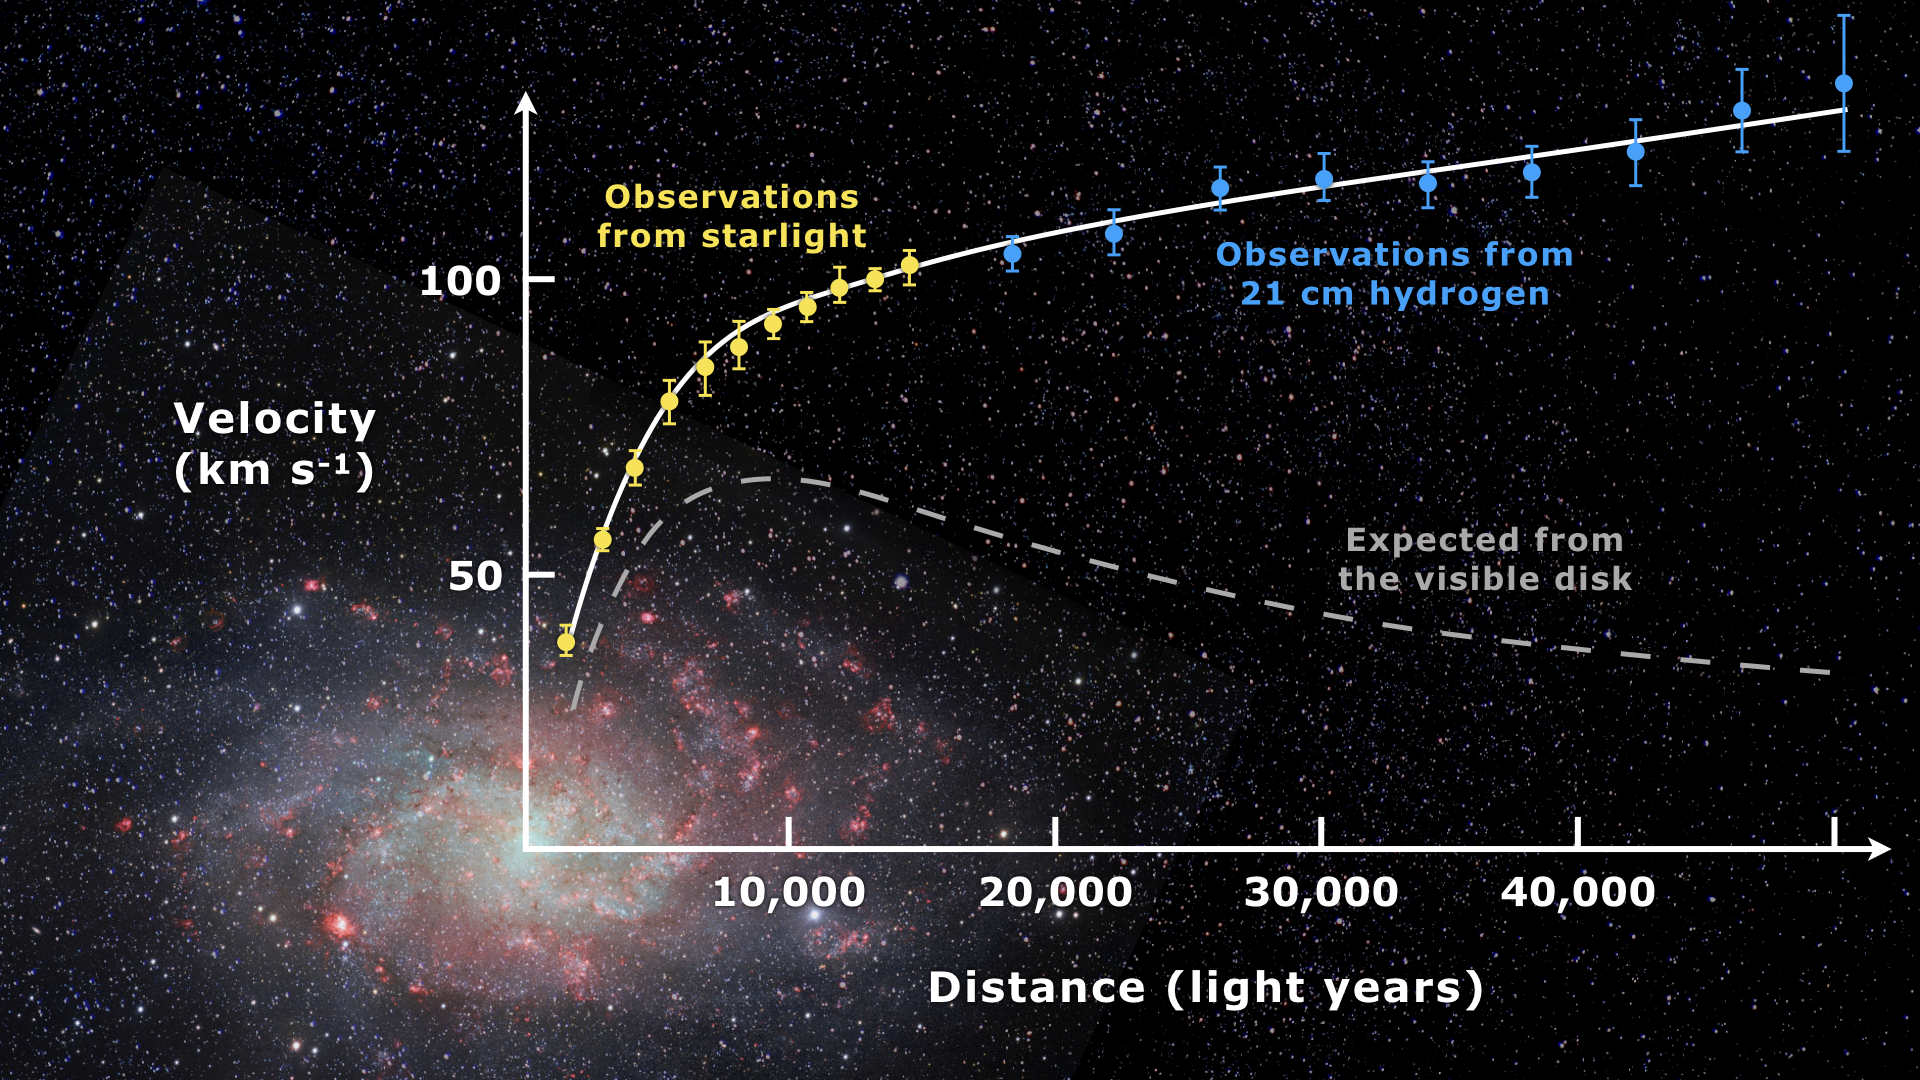
\includegraphics[width=.9\textwidth]{figures/Rotation_curve_galaxy.png}
		\caption{Courbe de rotation de la galaxie spirale Messier 33 \\ \credits{Wikipedia}}
	\end{figure}
\end{column}
\begin{column}{0.5\textwidth}
	\begin{figure}
		\centering
		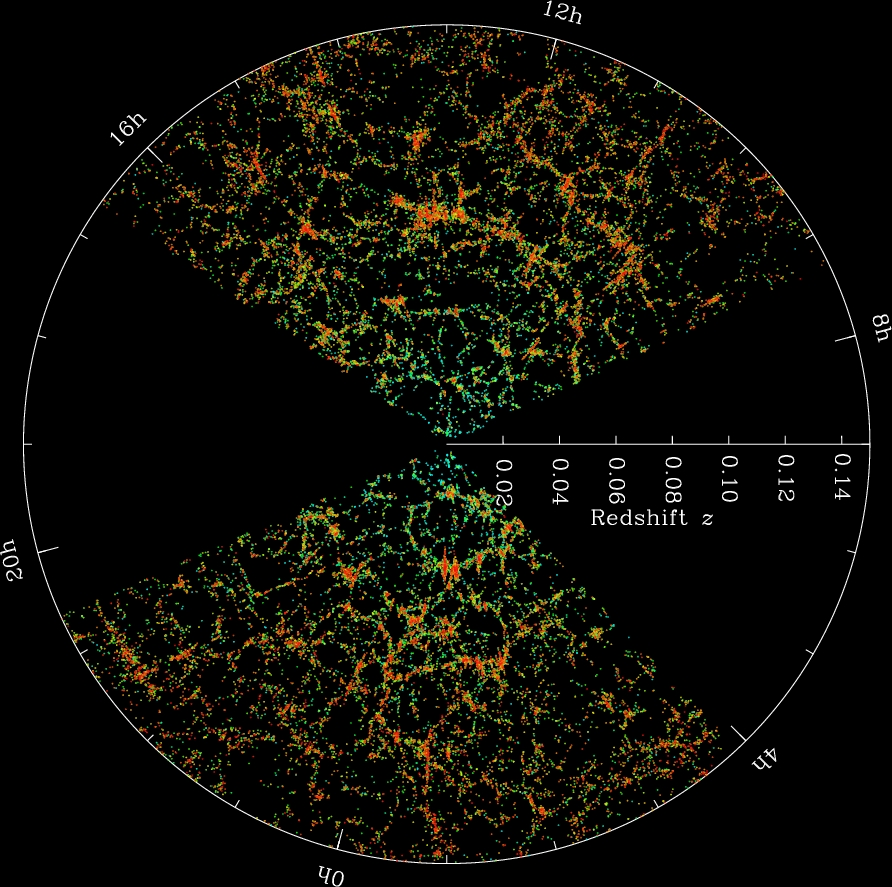
\includegraphics[width=.8\textwidth]{figures/sdss_pie2.jpg}
		\caption{Distribution des galaxies observées par le Sloan Digital Sky Survey \\ \credits{M. Blanton and the Sloan Digital Sky Survey}}
	\end{figure}
\end{column}
\end{columns}
\end{frame}

\begin{frame}{Energie noire et SNe Ia}
\begin{columns}
\begin{column}{0.6\textwidth}
	\begin{itemize}
\item L'énergie noire a été introduite pour expliquer l'accélération de l'expansion de l'univers.
\item	Cette accélération a été découverte à l'aide de SNeIa par S. Perlmutter, B. Schmidt et A. Riess
\item Magnitudes décrites par la formule de Tripp
\begin{equation}
	M^*_{b,SN} = M_b - \alpha x_{1,SN} + \beta c_{SN} + n(\sigma_{int})
\end{equation}
\end{itemize}
\end{column}
\begin{column}{0.4\textwidth}
	\begin{figure}
		\centering
		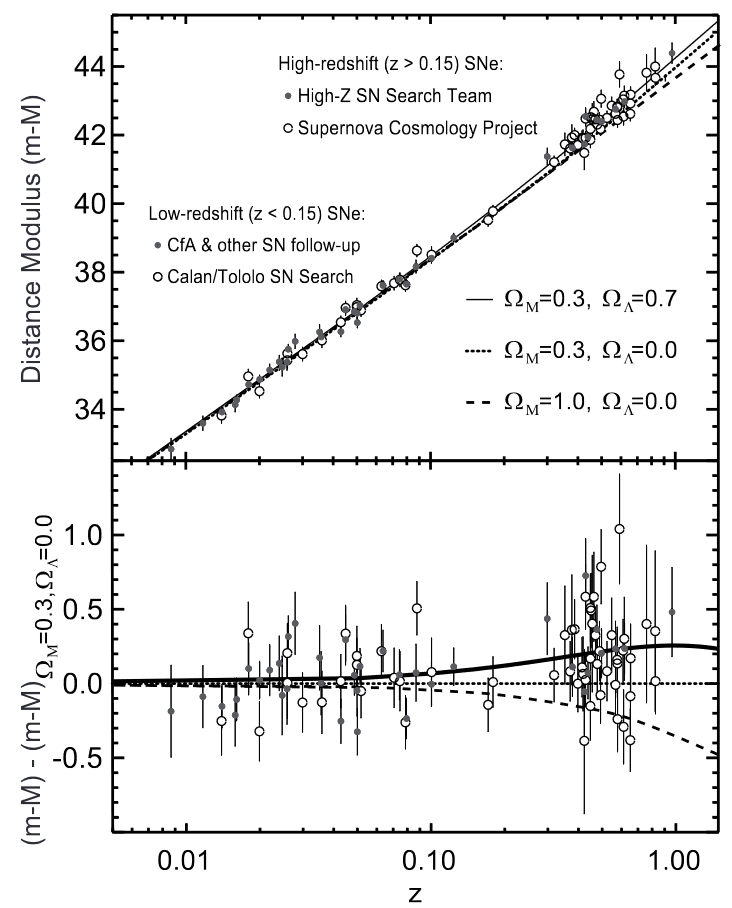
\includegraphics[height=0.6\textheight]{figures/Perlmutter_Schmidt.png}
		\caption{Diagramme de Hubble construit par Perlmutter et Schmidt en 2003}
	\end{figure}
\end{column}
\end{columns}
\end{frame}

\subsection{DESI}

\begin{frame}{Dark Energy Spectroscopic Instrument}
\begin{columns}
\begin{column}{.5\textwidth}
	\begin{itemize}
		\item Utilise le Mayall Telescope à l'Observatoire de Kitt peak 
		\item 4m de diamètre pour un champ de 8.0 degrés carré
		\item 5 000 fibres robotisées
		\item $\sim 30$ millions de galaxies ciblées
	\end{itemize}
	\begin{figure}
		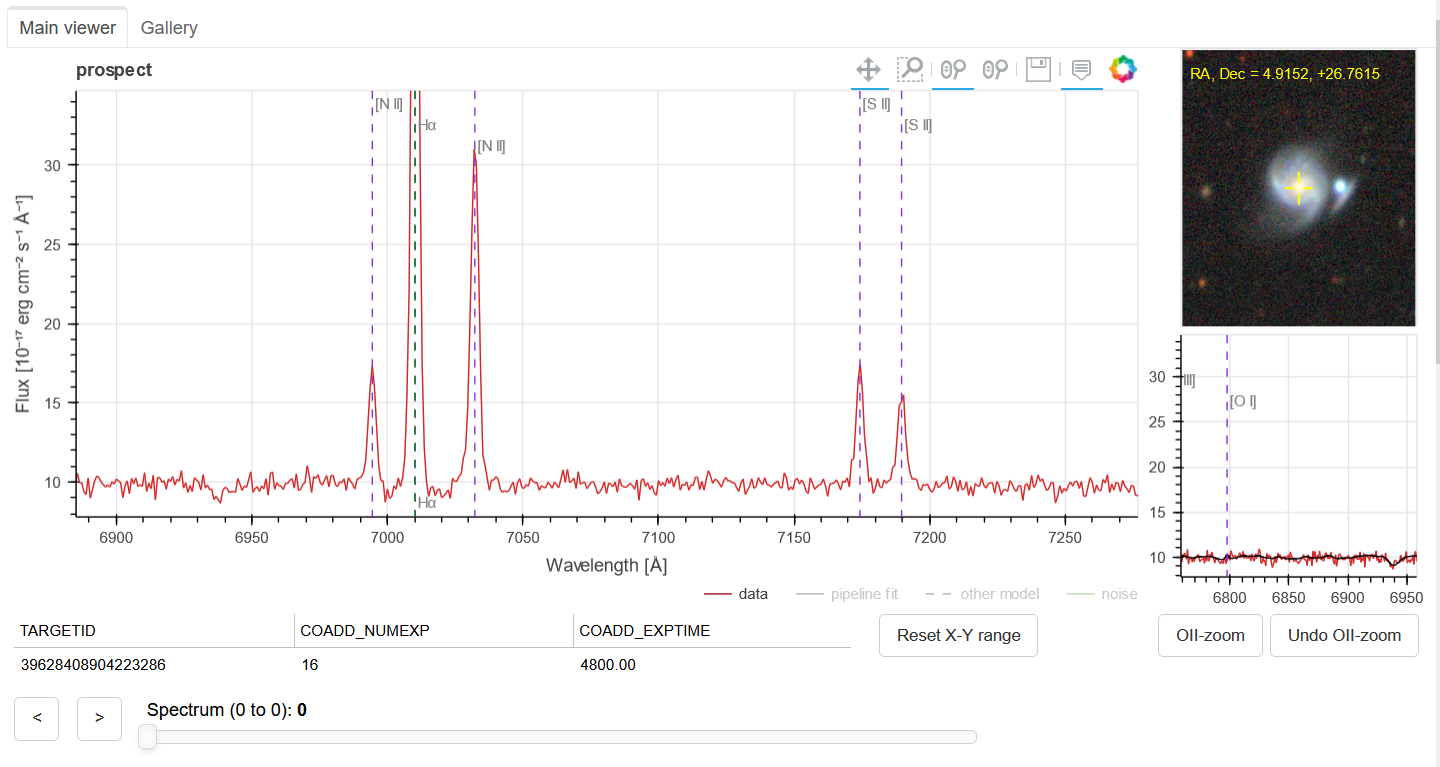
\includegraphics[height=2cm]{figures/DESI_spec.png}
		\caption{Exemple de spectre observé par DESI \credits{Wikipedia}}
	\end{figure}
\end{column}

\begin{column}{.5\textwidth}
	\begin{figure}
		\centering
		\includegraphics[width=0.6\textwidth]{figures/Artistic_DESI.jpg}
		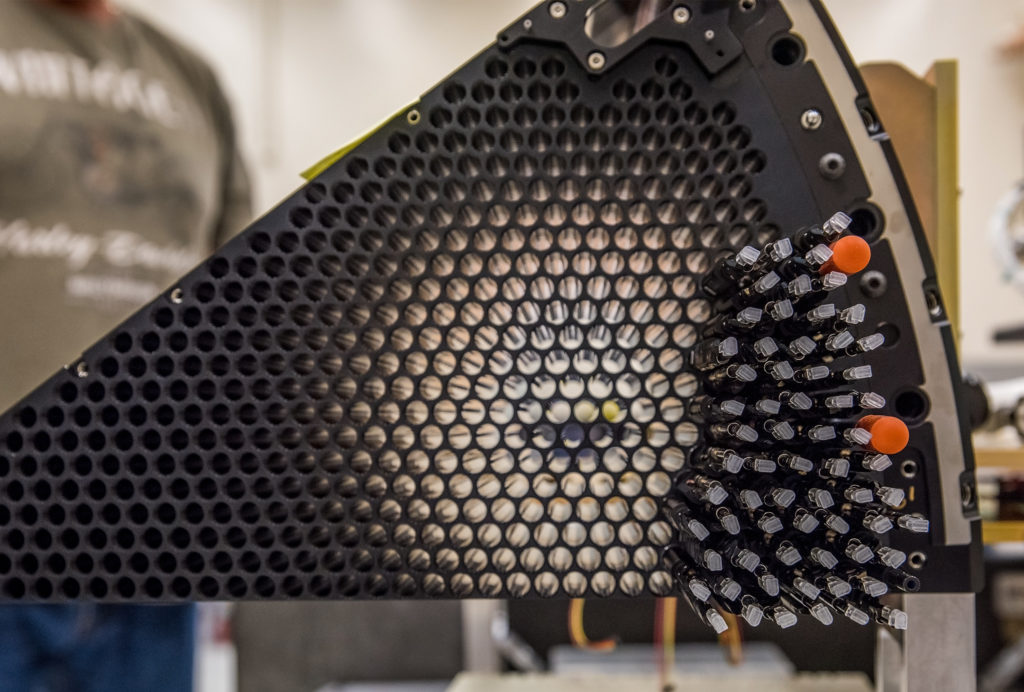
\includegraphics[width=0.6\textwidth]{figures/DESI_focal_plane.jpg}
		\caption{Vue d'artiste du Mayall Telescope avec les données DESI Y1 et plan focal supportant les robots\\ \credits{DESI Collaboration/KPNO/NOIRLab/NSF/AURA/P. Horálek/R. Proctor}}
	\end{figure}
\end{column}
\end{columns}
\end{frame}

\subsection{ZTF}
\begin{frame}{ZTF}
\begin{columns}
\begin{column}{.5\textwidth}
	\begin{itemize}
		\item Situé à l'Observatoire de Palomar, utilise le telescope P48
		\item 1,22m de diamètre pour un champ de 47 degrés carré
		\item 16 CCDs de $6144 \times 6160$ pixels
		\item Couvre le ciel de l'hémisphère nord deux fois par nuit
	\end{itemize}
\end{column}

\begin{column}{.5\textwidth}
	\begin{figure}
		\centering
		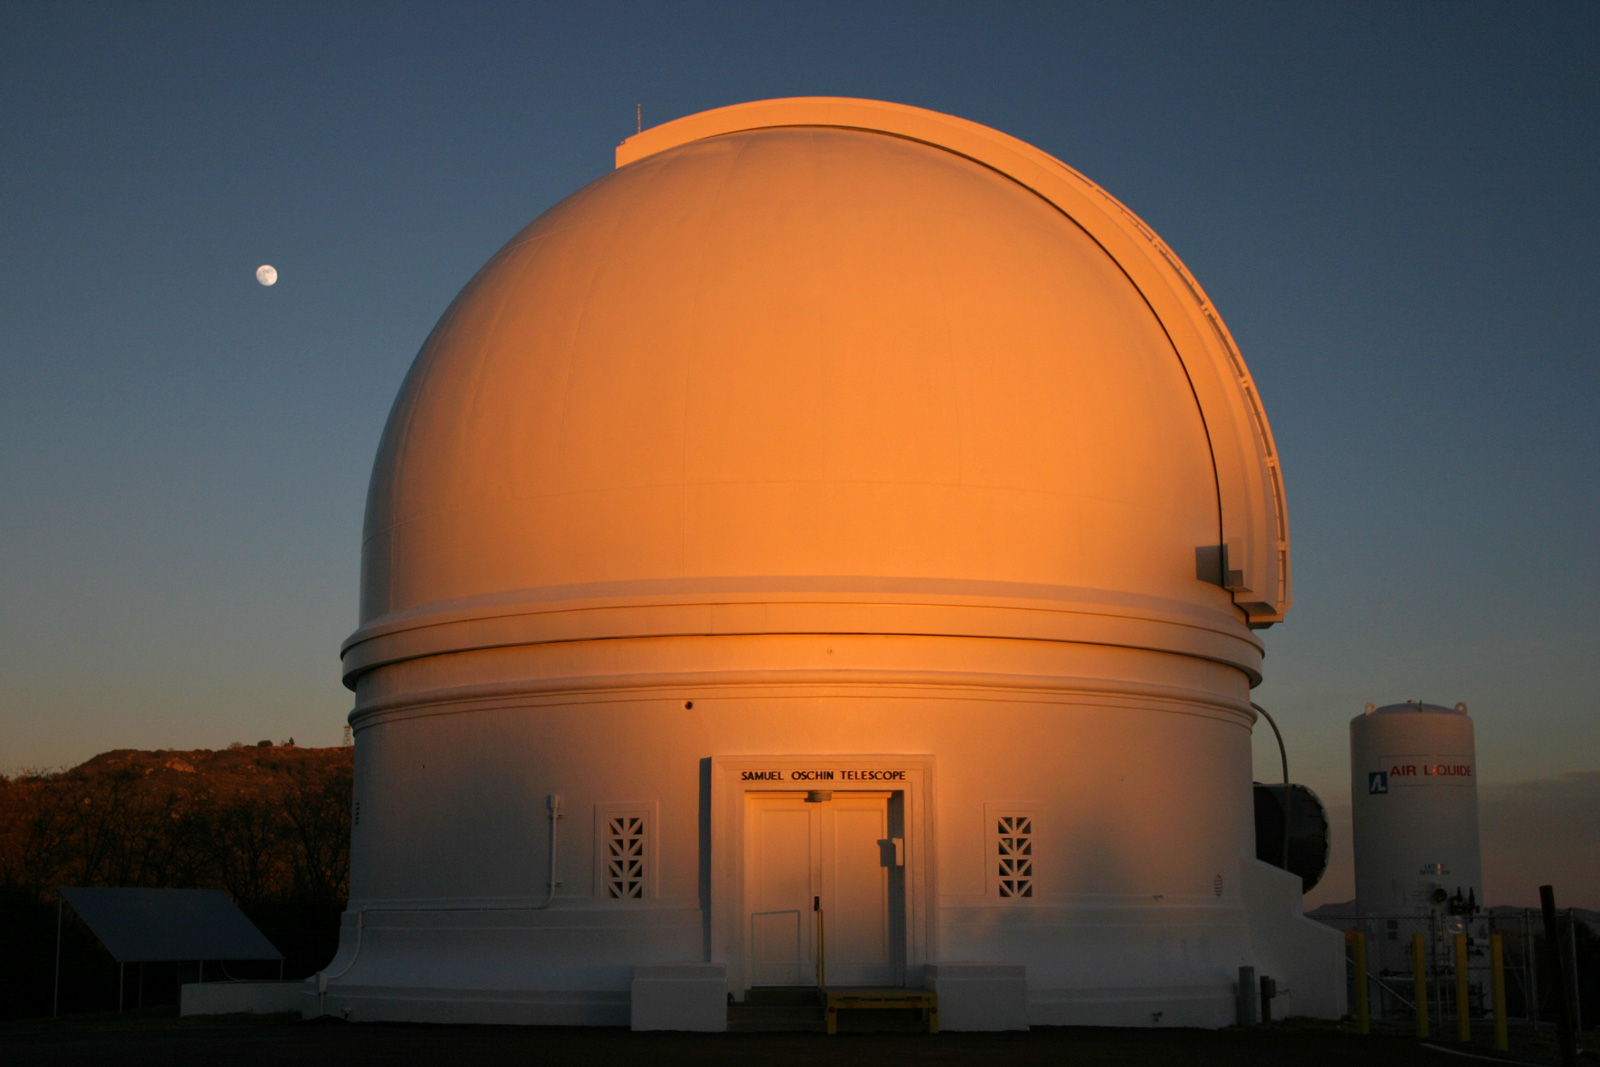
\includegraphics[width=.5\textwidth]{figures/ZTF_dome.jpg}
		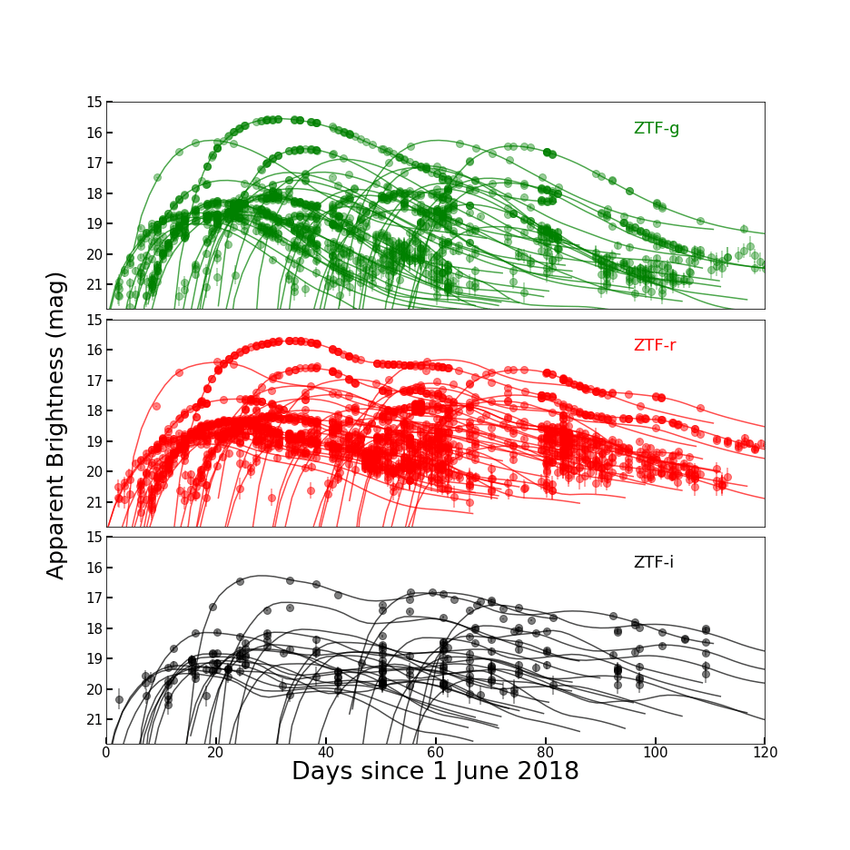
\includegraphics[width=.6\textwidth]{figures/ZTF_lightcurves.png}
		\caption{Telescope P48 utilisé par ZTF et exemples de courbes de lumière de SNe Ia \\ \credits{Caltech/Palomar}}
	\end{figure}
\end{column}
\end{columns}
\end{frame}

\subsection{Croissances des structures}

\begin{frame}{Croissance des structures dans l'Univers}
	Taux de croissance des structues~: $f(z)$
	\begin{figure}
		\centering
		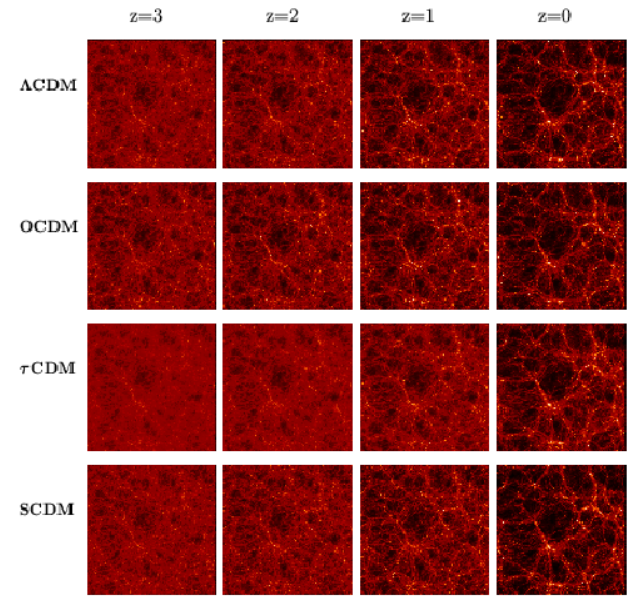
\includegraphics[height=0.6\textheight]{figures/struct_growth.png}
		\caption{Formation des structures pour différents modèles\\ \credits{Kauffmann, Colberg, Diaferio, and White}}
	\end{figure}
\end{frame}

\begin{frame}{Observations}
\begin{figure}
	\centering
	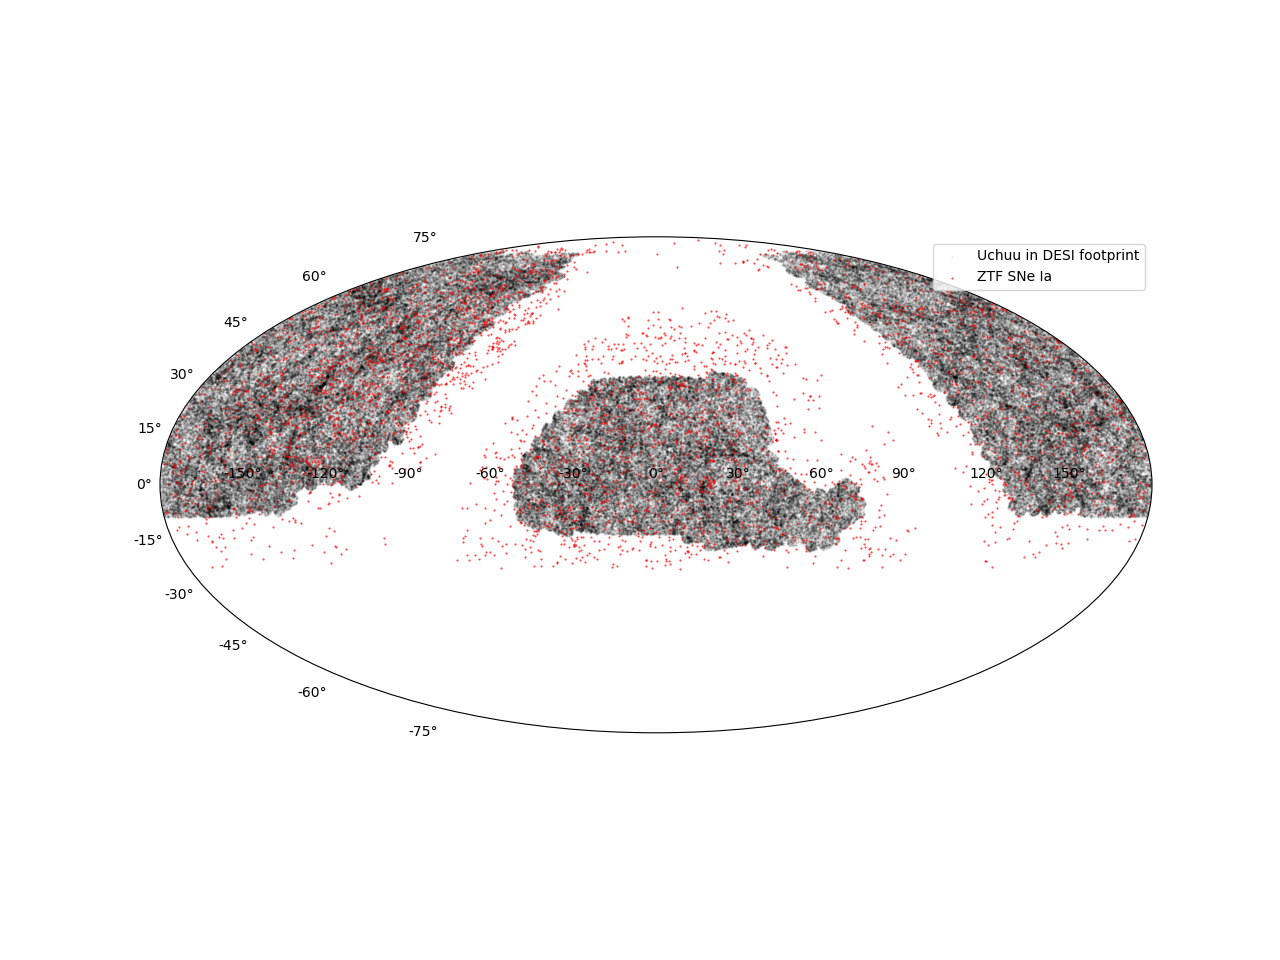
\includegraphics[width=0.9\textwidth, trim = {3cm, 5cm, 2cm, 5cm}, clip]{figures/ZTF_on_DESI.png}
	\caption{SNe Ia issues de la DR1 de ZTF et footprint DESI}
\end{figure}
\end{frame}

\begin{frame}{Redshift Space Distortion et clustering des galaxies}
	Les vitesses particulières des galaxies sont proportionnelles à $f(z) \sigma_8(z)$ et décalent le redshift observé
	\begin{equation}
		z_{obs} = (1+z_{cosmo}) (1 + z_{pec}) = (1+z_{cosmo}) \qty(1 + \frac{1}{c} \vb v_{pec} \cdot \vu r)
	\end{equation}
	\begin{figure}
		\centering
		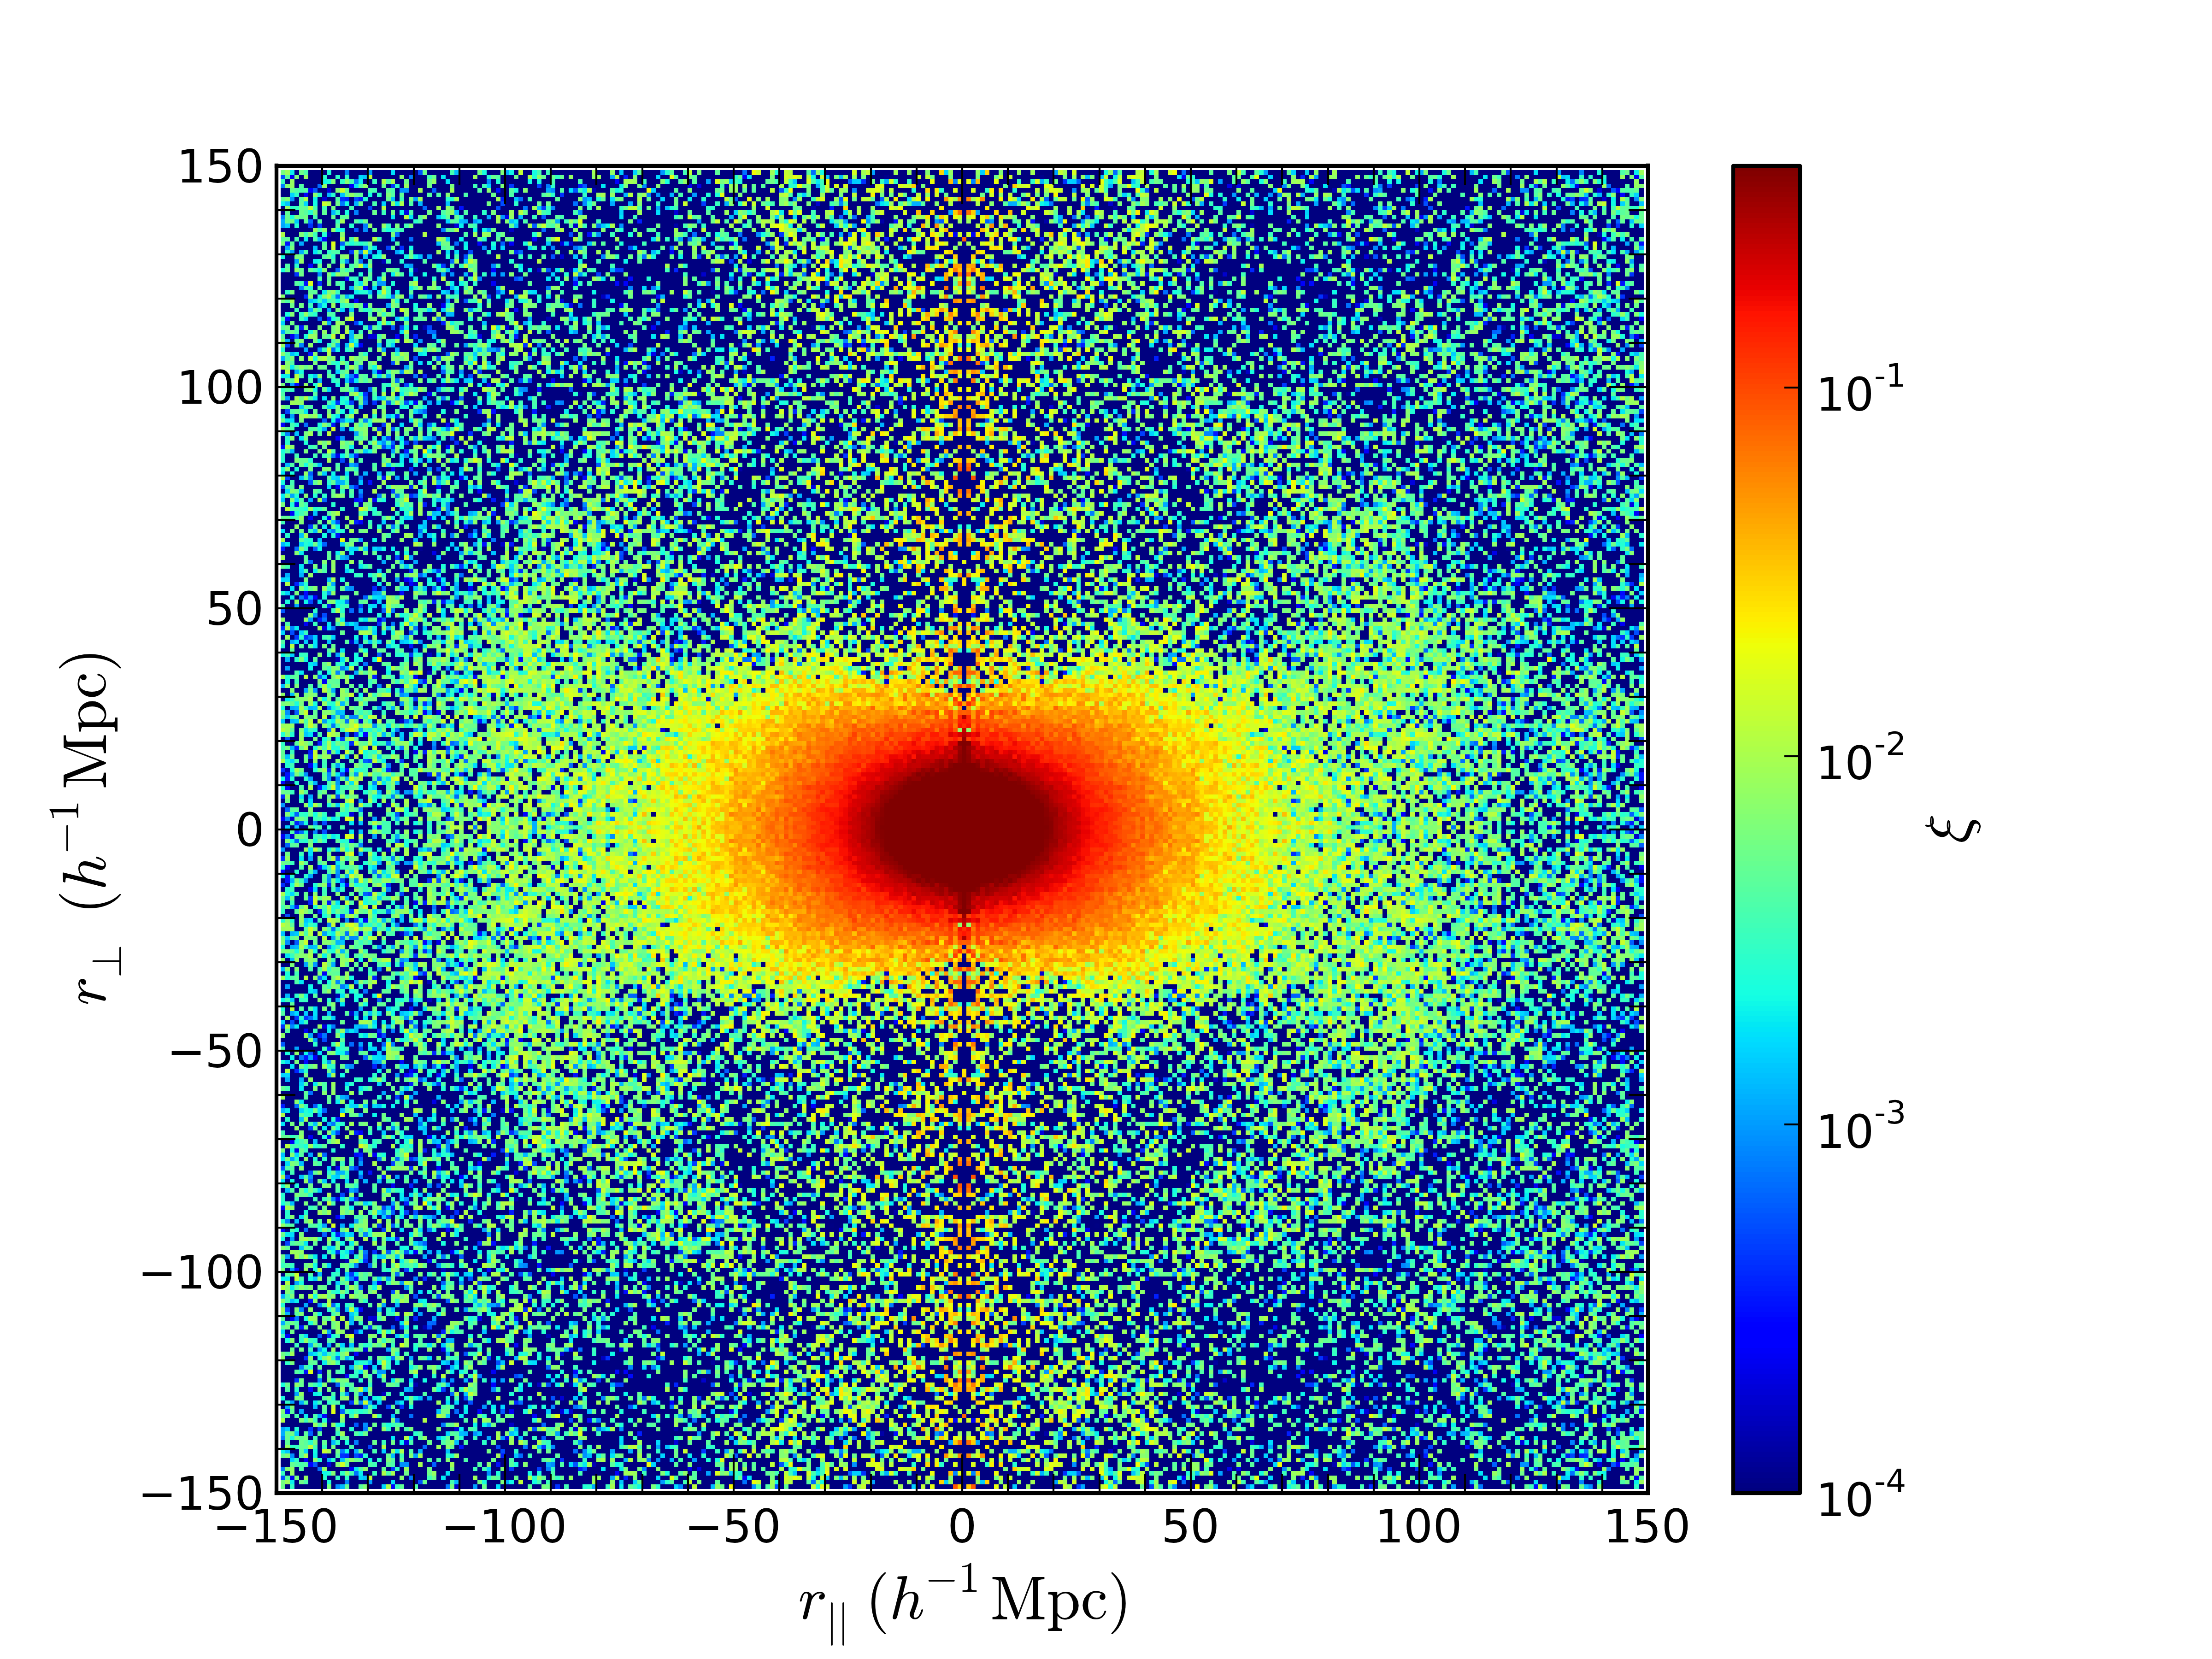
\includegraphics[height=0.5\textheight]{figures/FoG.png}
		\caption{Fonction de corrélation 2D des galaxies du relevé DR11 CMASS\\ \credits{SDSS Collaboration, Samushia et al. (2013)}}
	\end{figure}
\end{frame}
		
\begin{frame}{Analyse jointe entre galaxies et SNe Ia}
\begin{figure}
	\centering
	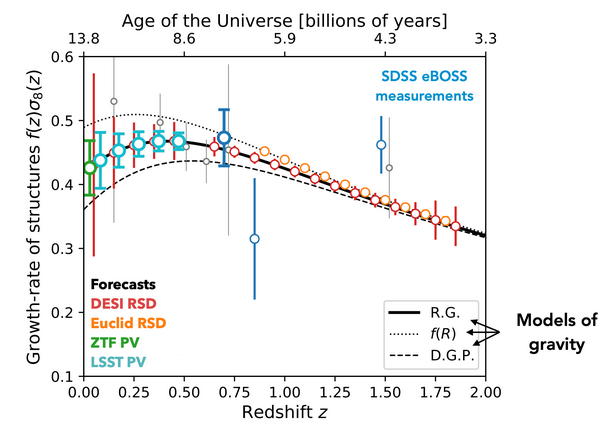
\includegraphics[height=0.7\textheight]{figures/fs8.png}
	\caption{Gain apporté par les vitesses particulières des SNe sur $f\sigma_8$}
\end{figure}
\end{frame}



\begin{frame}{Objectifs du stage}
\begin{enumerate}
\itemsep2em 
\item Générer des supernovae incluant des effets de vitesses particulières
\item Permettre un test du pipeline \lemaitre
\item Reconstruire les vitesses particulières des SNe Ia en vu d'une analyse $f\sigma_8$
\end{enumerate}
\end{frame}

\section{Chaîne d'analyse cosmologique avec SNe Ia}


% Suivre la reconstruction d'une SNe

\subsection{Générations des SNe}

\begin{frame}{Générations des SNe}
\begin{columns}
\begin{column}{.5\textwidth}
Paramètres des SNe selon les distributions usuelles
\begin{figure}
	\centering
	\alt<2>{
	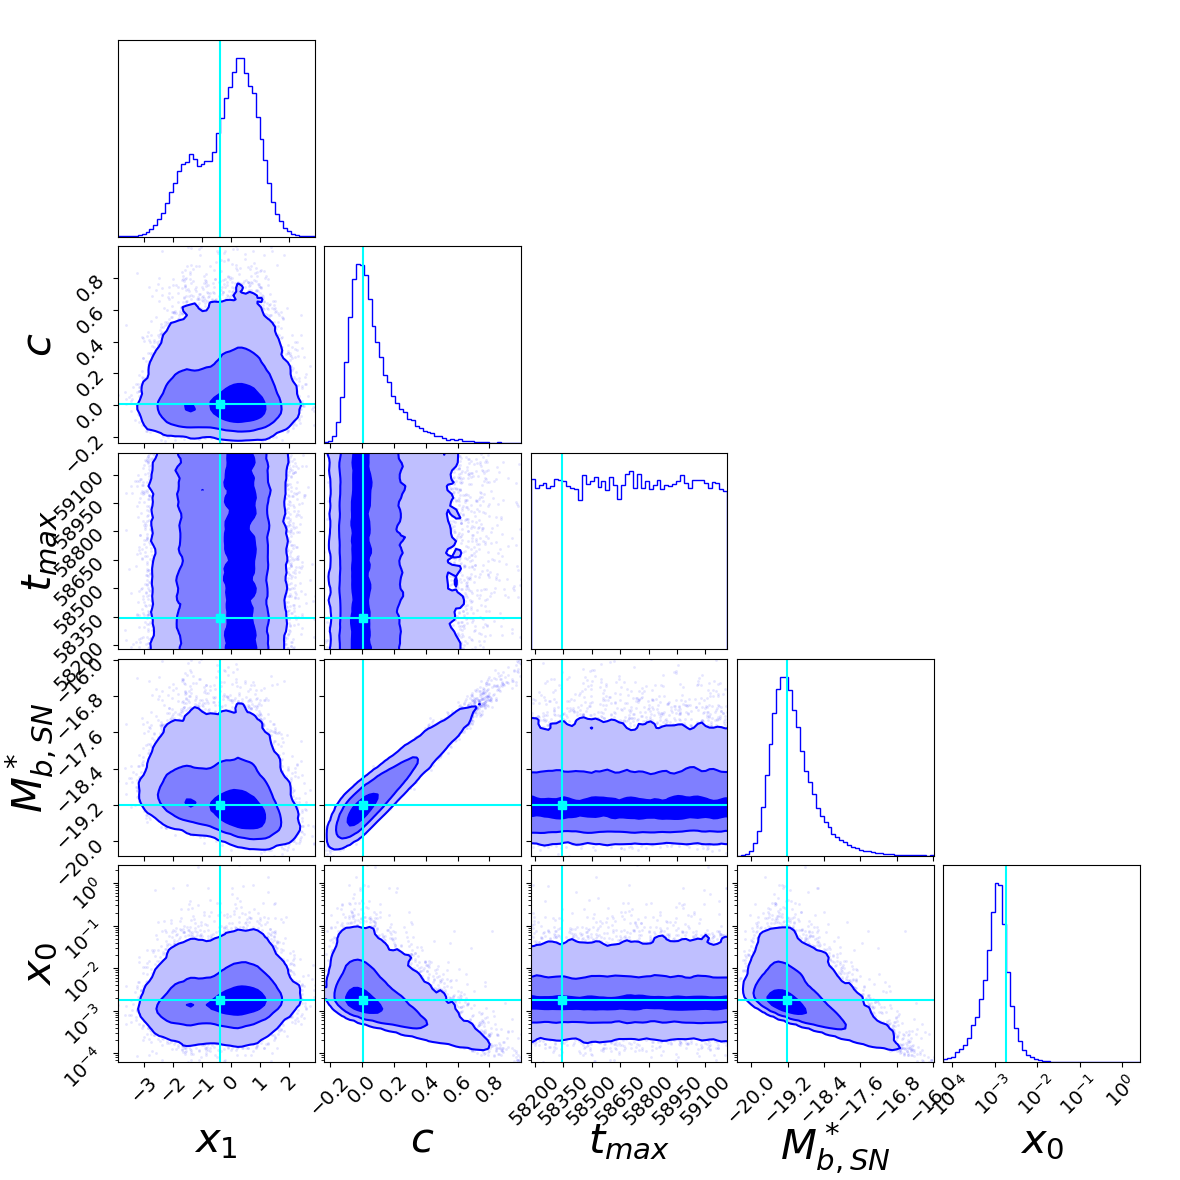
\includegraphics[height=4cm]{figures/SNe_sampling_pt.png}}
	{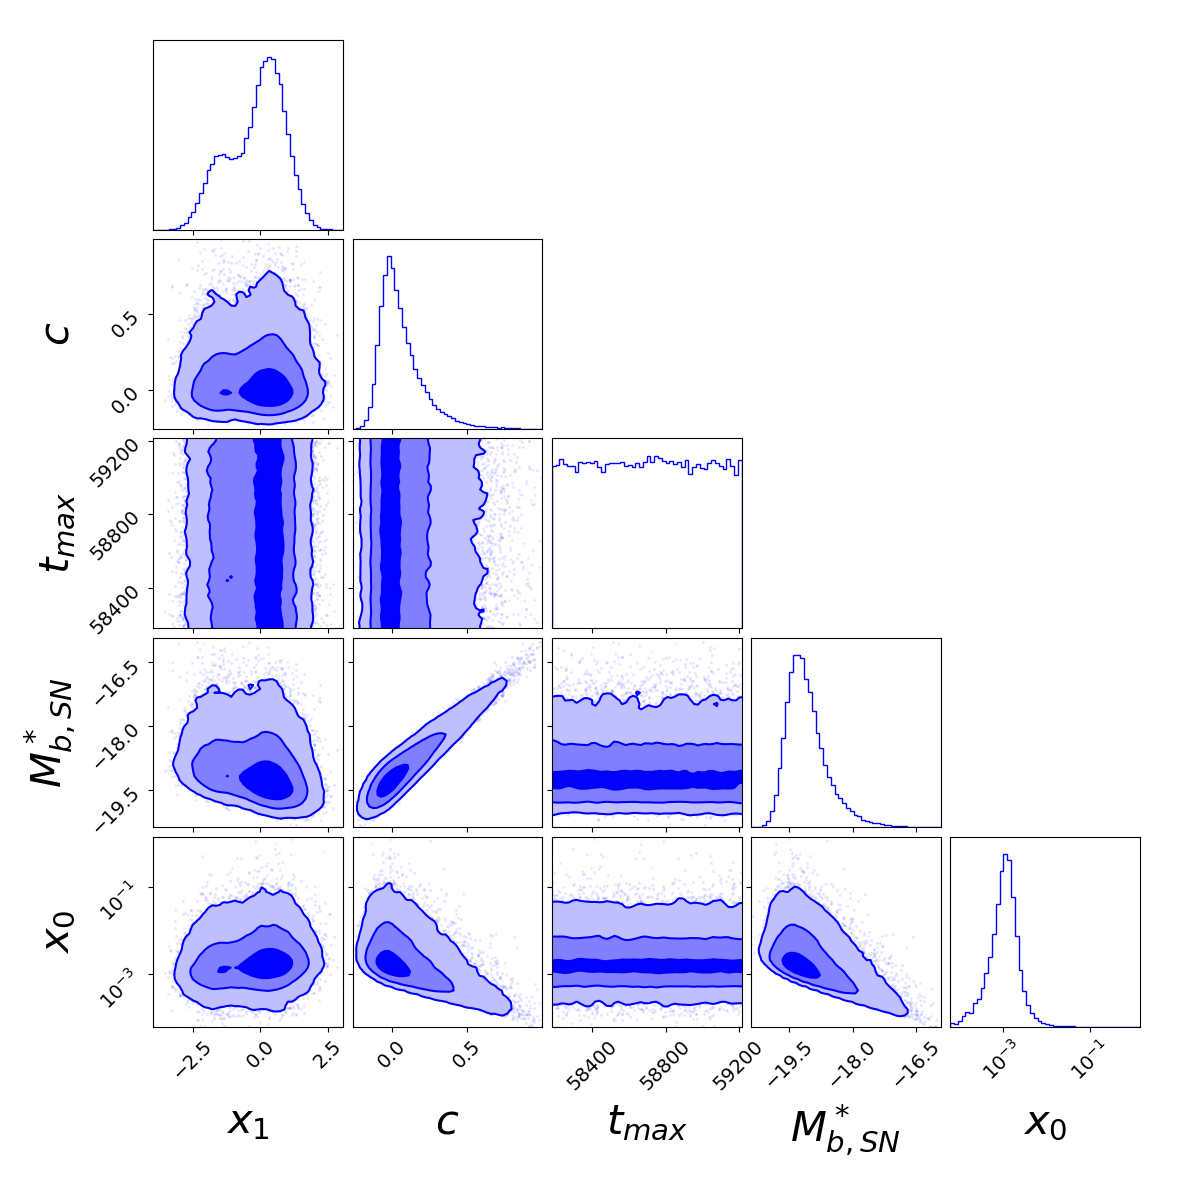
\includegraphics[height=4cm]{figures/SNe_sampling.png}}
	\caption{Distribution des paramètres des SNe}
\end{figure}
\end{column}

\begin{column}{.5\textwidth}
Position $(ra, dec, z)$ uniformément dans Uchuu BGS ($z < 0.06$)
\begin{figure}
	\centering
	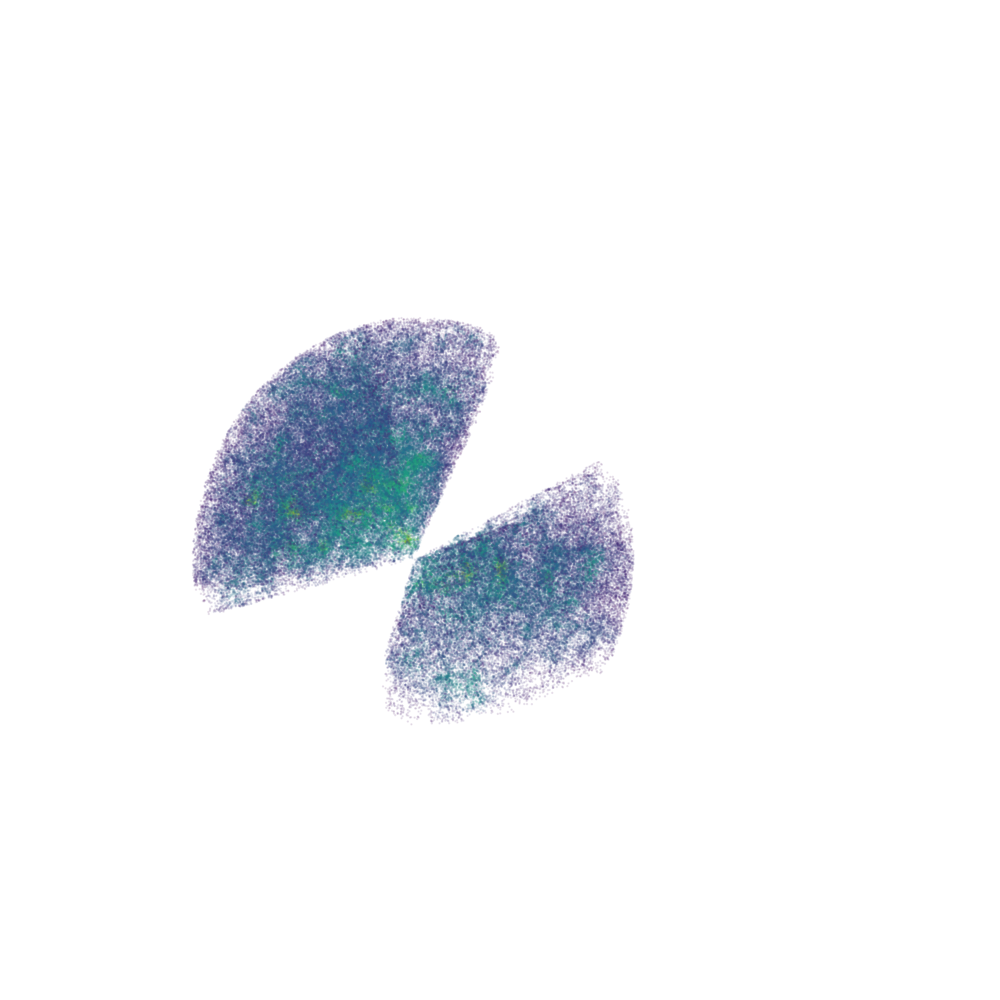
\includegraphics[height=4cm, trim={3cm 5cm 55mm 6cm}, clip]{figures/Uchuu.png}
	\caption{Distributions des galaxies du Uchuu BGS}
\end{figure}
\end{column}
\end{columns}
\end{frame}

\begin{frame}{Courbes de lumière et spectres}
\begin{columns}
\begin{column}{.5\textwidth}
\begin{figure}
	\centering
	\alt<2-3>{
	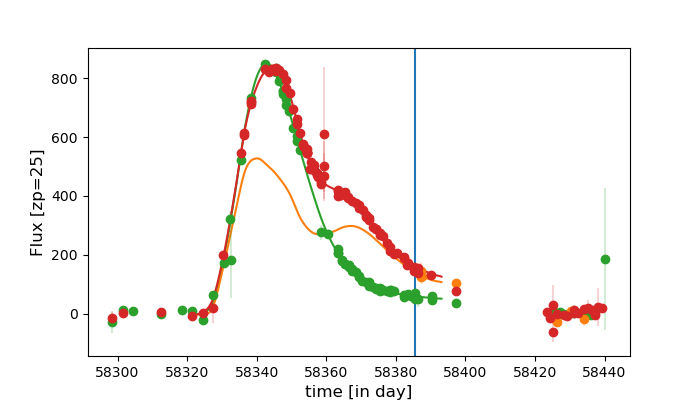
\includegraphics[width=.9\textwidth]{figures/26_lc_pt.png}}
	{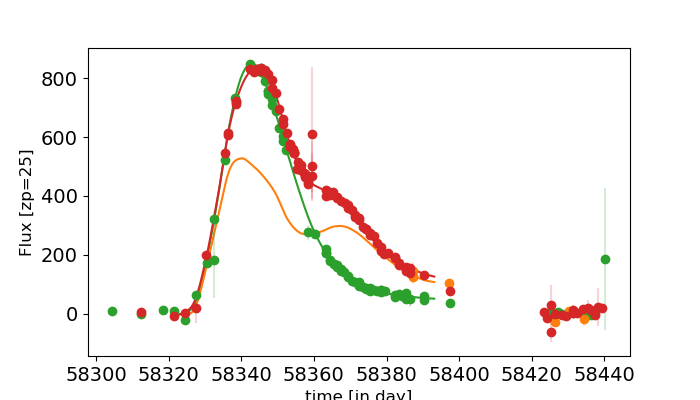
\includegraphics[width=.9\textwidth]{figures/26_lc.png}}
	\caption{Courbes de lumière de la SNe tirée}
\end{figure}
\end{column}

\begin{column}{.5\textwidth}
\begin{figure}
	\centering
	\invisible<1-2>{
	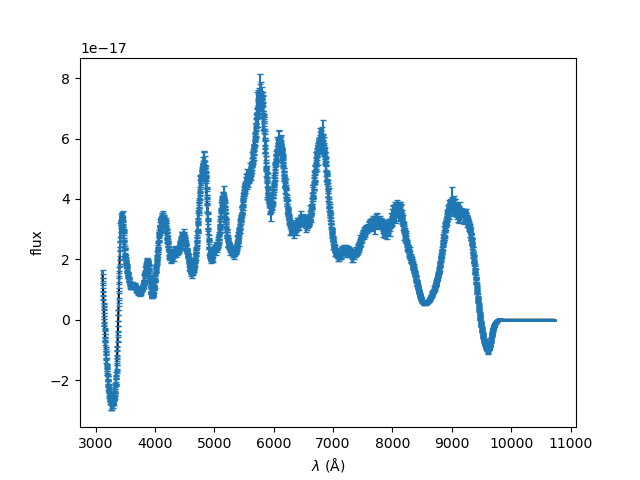
\includegraphics[width=.9\textwidth]{figures/26_spec.png}
	\caption{Spectre de la SNe tirée}}
\end{figure}
\end{column}
\end{columns}
\end{frame}

\subsection{Sélection par \texttt{PETS}}

\begin{frame}{Filtrage}
\begin{columns}
\begin{column}{.5\textwidth}
\begin{figure}
	\centering
	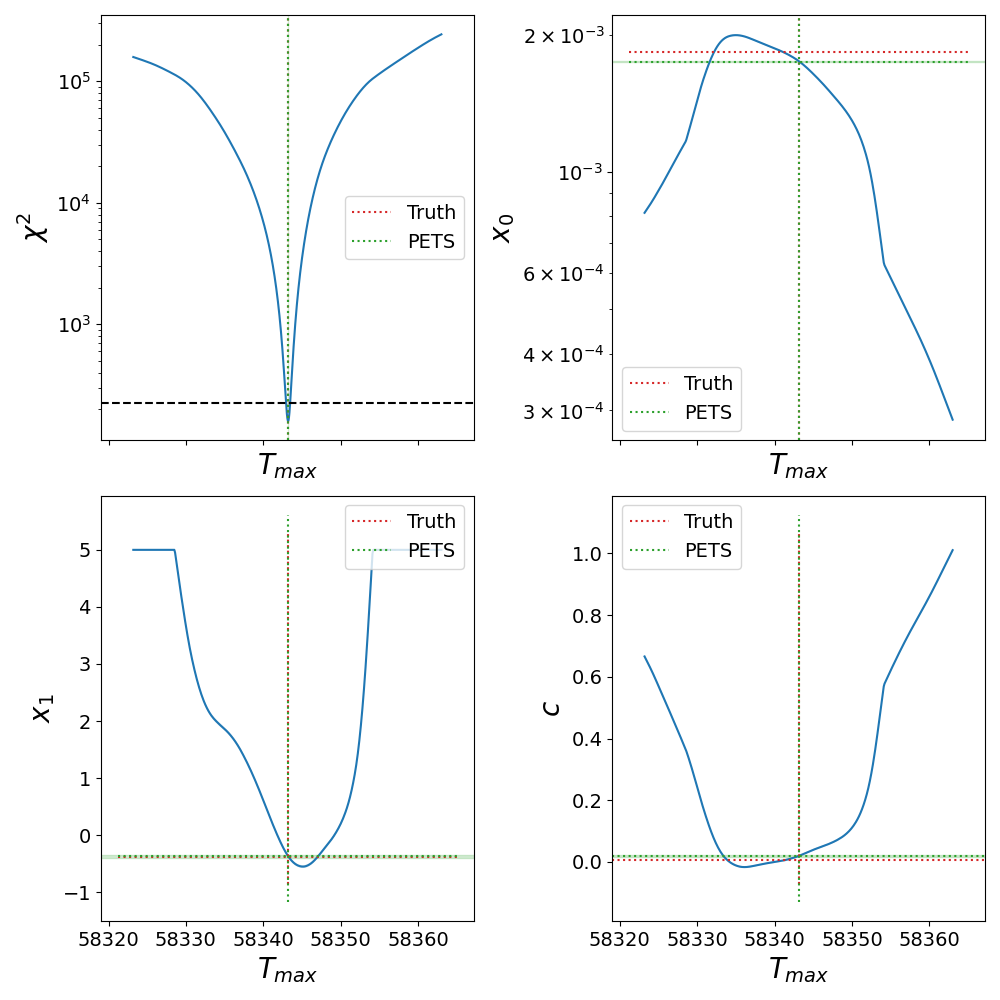
\includegraphics[width=.9\textwidth]{figures/26_pets_old.png}
	\caption{Variation des paramètres en fonction de $t_{max}$ utilisée par \texttt{PETS}}
\end{figure}
\end{column}

\begin{column}{.5\textwidth}
\begin{figure}
	\centering
	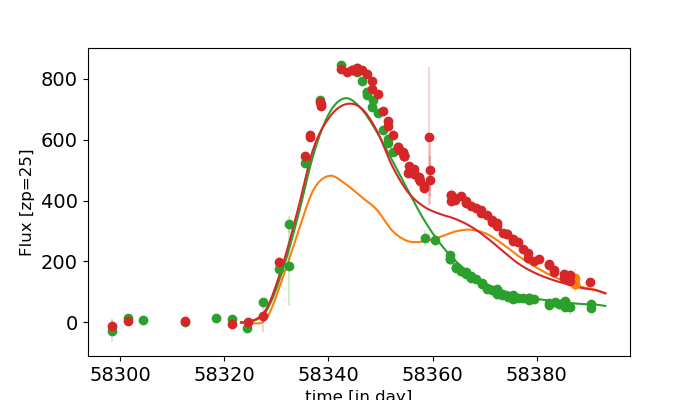
\includegraphics[width=.9\textwidth]{figures/26_lc_pets.png}
	\caption{Courbes de lumière obtenues par \texttt{PETS}}
\end{figure}
\end{column}
\end{columns}
\end{frame}

\begin{frame}{Après correction des cartes de poussières}
\begin{columns}
\begin{column}{.5\textwidth}
\begin{figure}
	\centering
	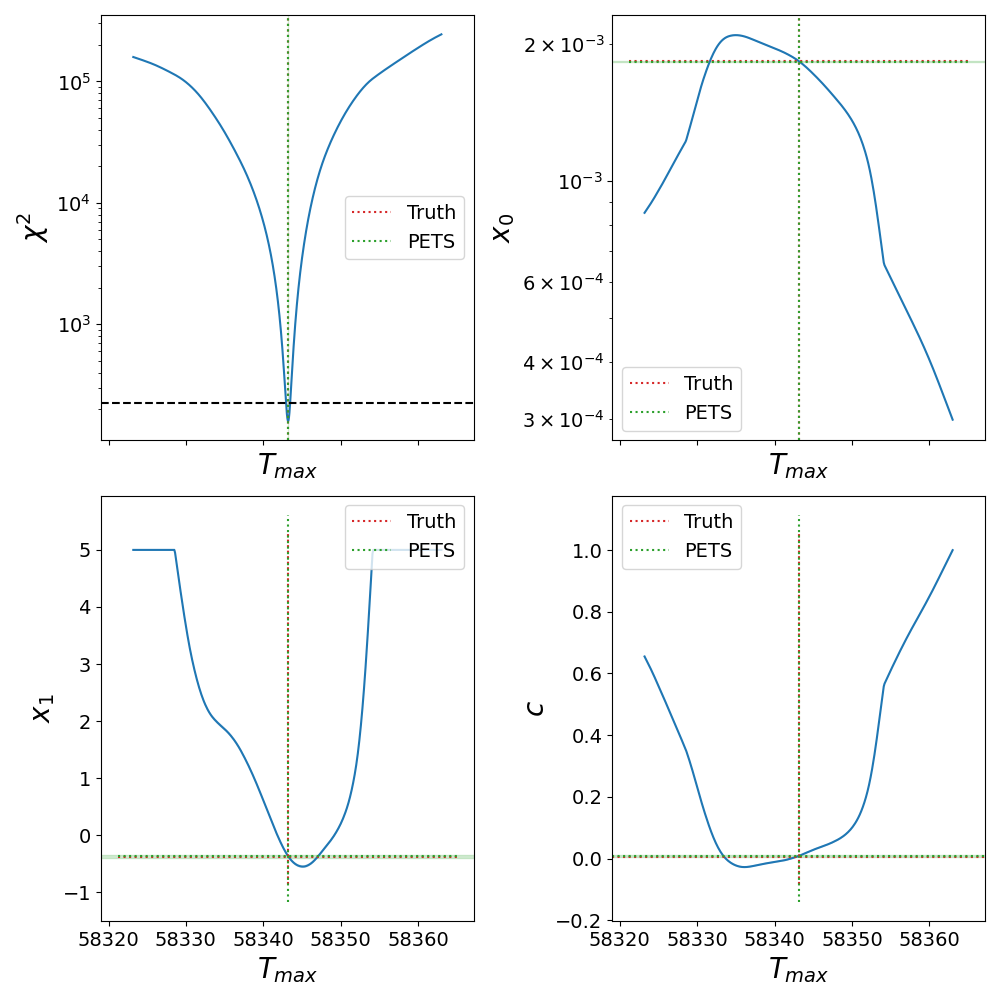
\includegraphics[width=.9\textwidth]{figures/26_pets_new.png}
	\caption{Variation des paramètres en fonction de $t_{max}$ utilisée par \texttt{PETS}}
\end{figure}
\end{column}

\begin{column}{.5\textwidth}
\begin{figure}
	\centering
	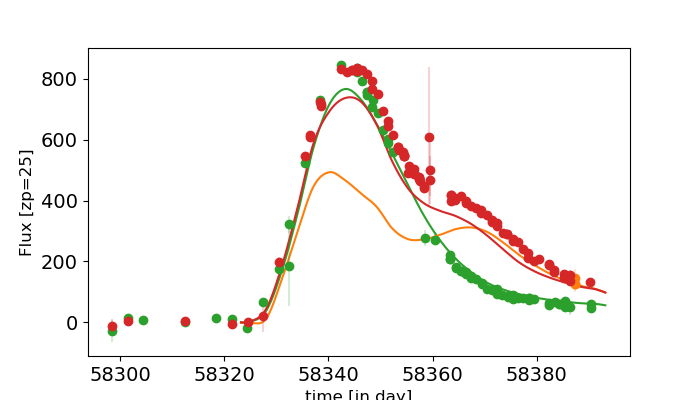
\includegraphics[width=.9\textwidth]{figures/26_lc_pets_new.png}
	\caption{Courbes de lumière obtenues par \texttt{PETS}}
\end{figure}
\end{column}
\end{columns}
\end{frame}


\subsection{Reconstruction des paramètres de standardisations}

\begin{frame}{\texttt{SALT2.4}}
\begin{figure}
	\begin{subfigure}{0.49\textwidth}
		\centering
		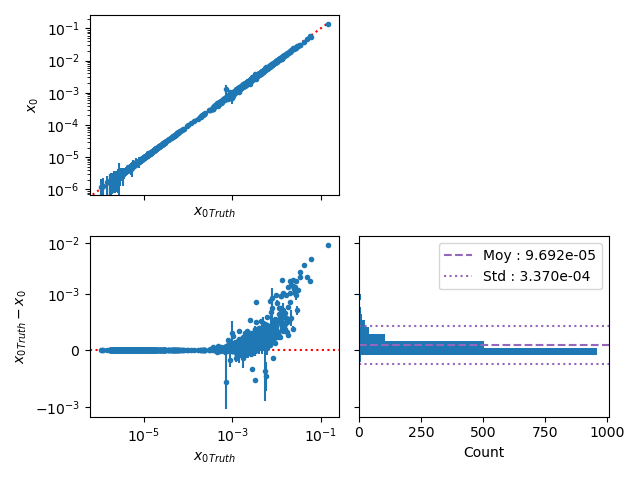
\includegraphics[width=.8\textwidth]{figures/salt_x0.png}
		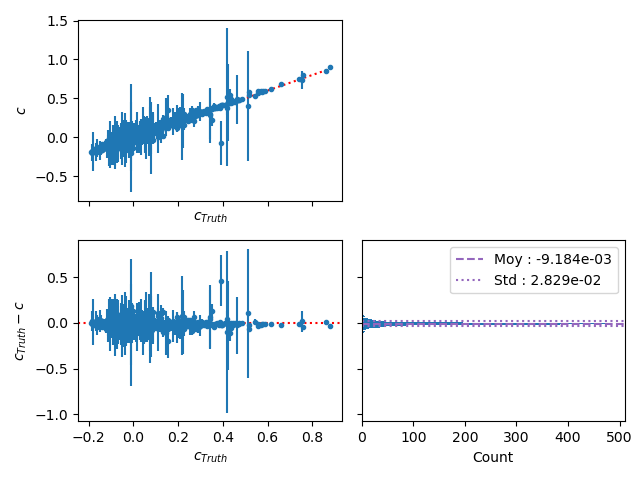
\includegraphics[width=.8\textwidth]{figures/salt_c.png}
	\end{subfigure}
	\begin{subfigure}{0.49\textwidth}
		\centering
		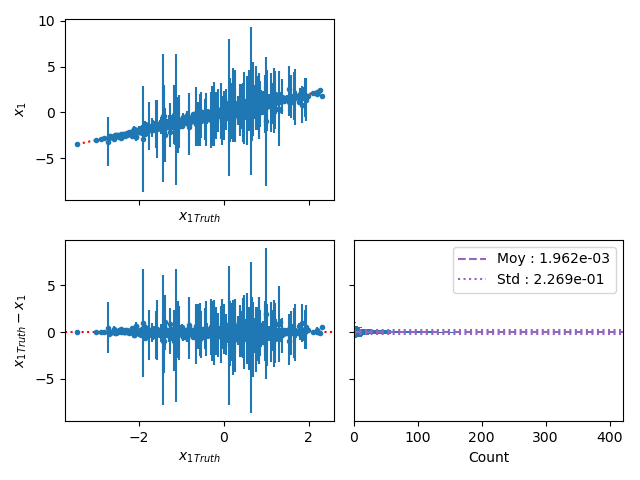
\includegraphics[width=.8\textwidth]{figures/salt_x1.png}
		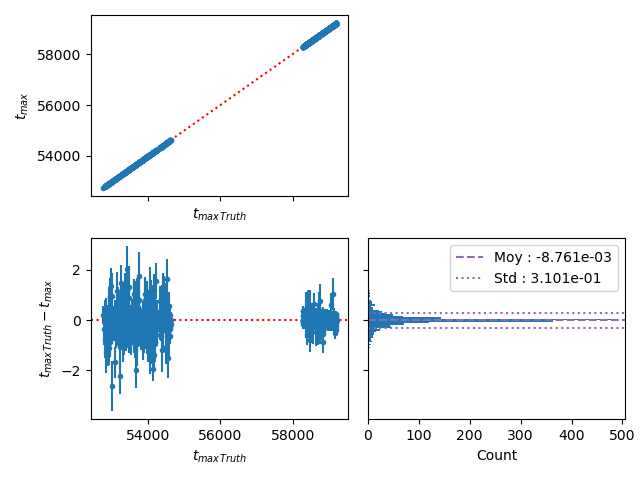
\includegraphics[width=.8\textwidth]{figures/salt_tmax.png}
	\end{subfigure}
	\caption{Paramètres de standardisations reconstruits par \texttt{SALT2.4}}
\end{figure}
\end{frame}

\begin{frame}{\texttt{NaCl}}
\begin{figure}
	\begin{subfigure}{0.49\textwidth}
		\centering
		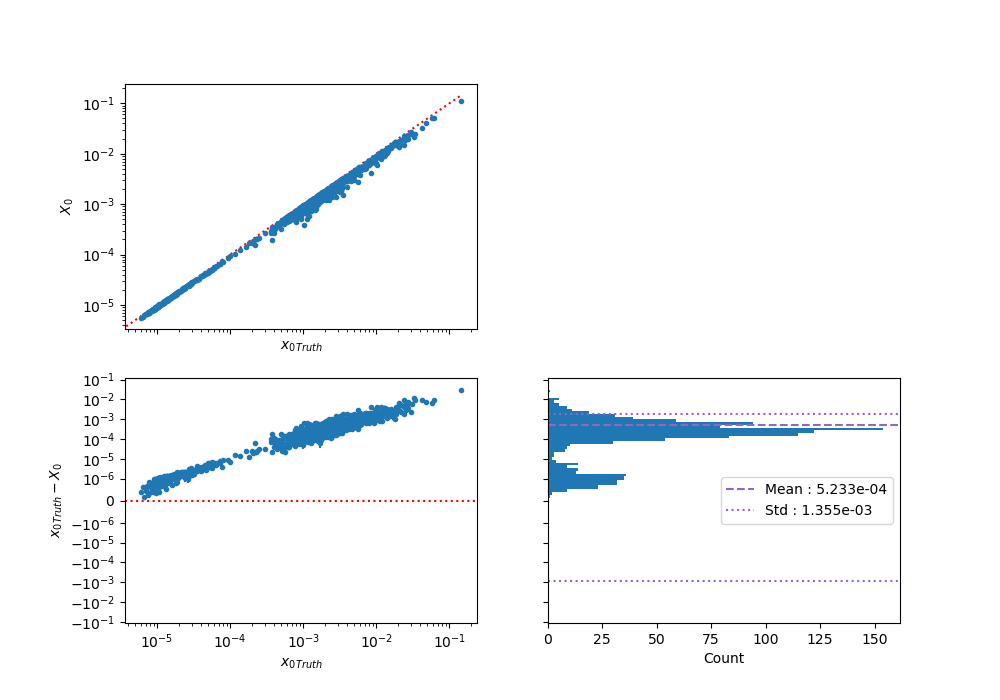
\includegraphics[width=.8\textwidth]{figures/nacl_x0.png}
		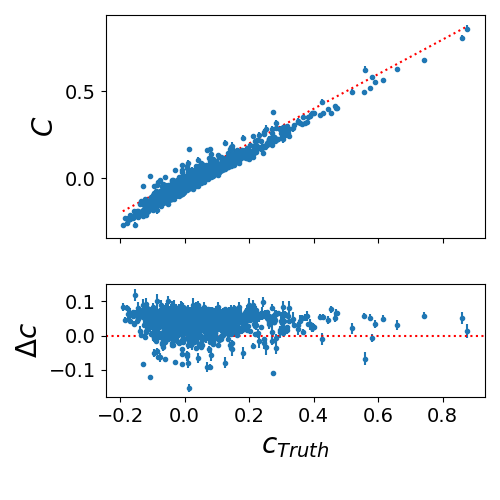
\includegraphics[width=.8\textwidth]{figures/nacl_c.png}
	\end{subfigure}
	\begin{subfigure}{0.49\textwidth}
		\centering
		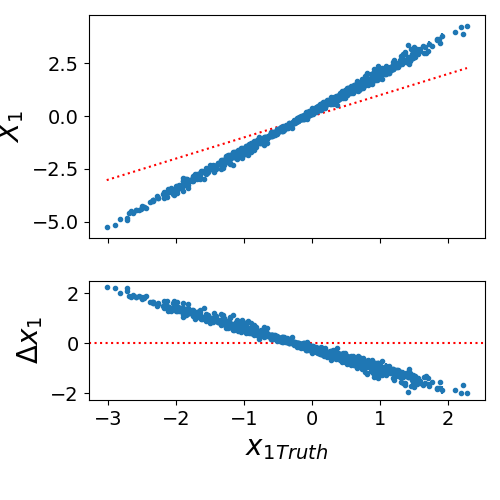
\includegraphics[width=.8\textwidth]{figures/nacl_x1.png}
		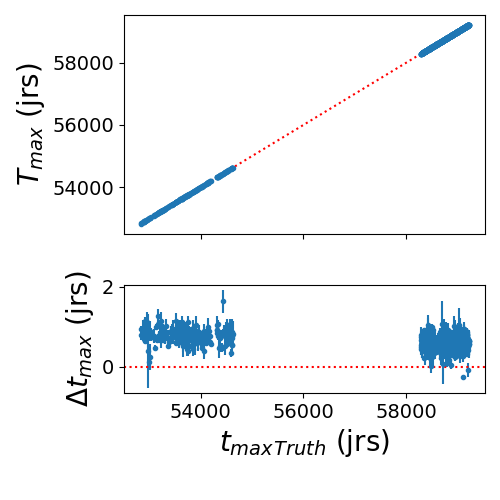
\includegraphics[width=.8\textwidth]{figures/nacl_tmax.png}
	\end{subfigure}
	\caption{Paramètres de standardisations reconstruits par \texttt{NaCl}}
\end{figure}
\end{frame}

\begin{frame}{Première estimation des distances à partir des paramètres de standardisation}
En supposant $\alpha=0.14$ et $\beta=3.15$ dans la formule de Tripp, on obtient
\begin{figure}
	\centering
	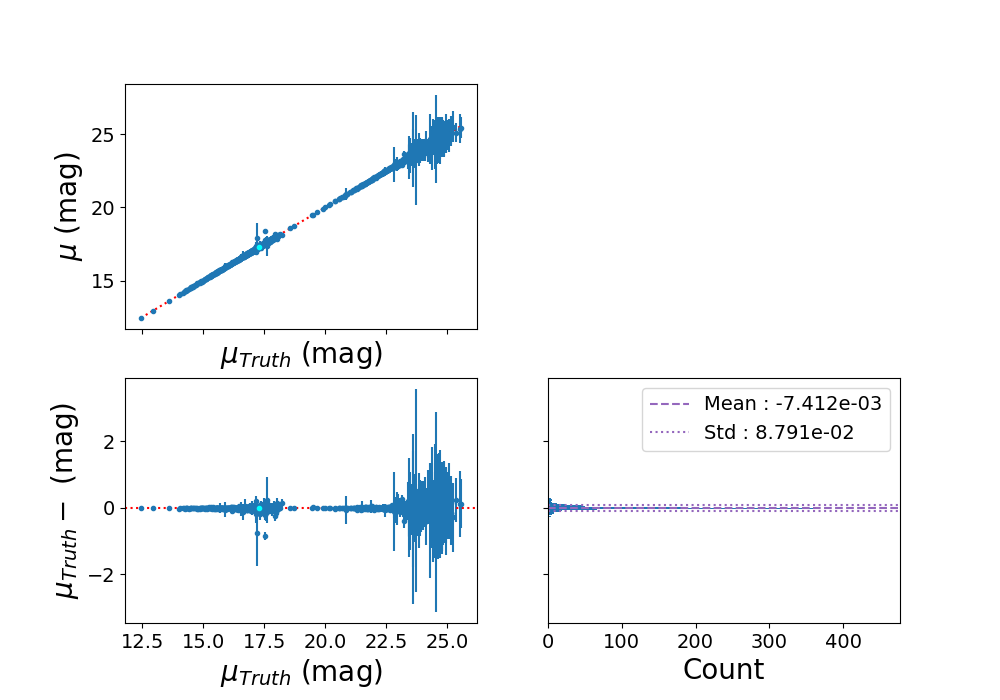
\includegraphics[width=.48\textwidth]{figures/salt_mu.png}
	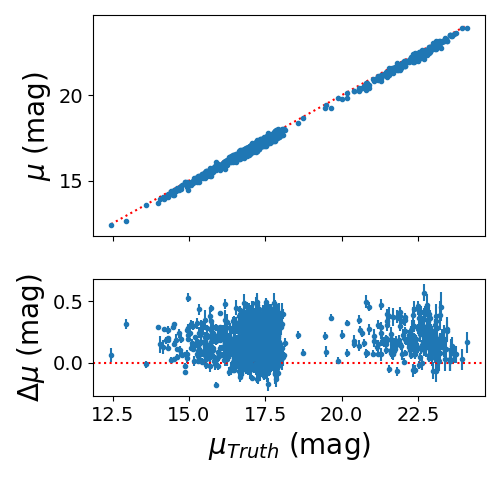
\includegraphics[width=.48\textwidth]{figures/nacl_mu.png}
	\caption{Modules de distance déterminés en utilisant \texttt{SALT2.4} (gauche) et \texttt{NaCl} (droite)}
\end{figure}
\end{frame}

\subsection{Reconstruction des distances et de la cosmologie}

\begin{frame}{Reconstruction des distances et de la cosmologie}
\begin{figure}
	\centering
	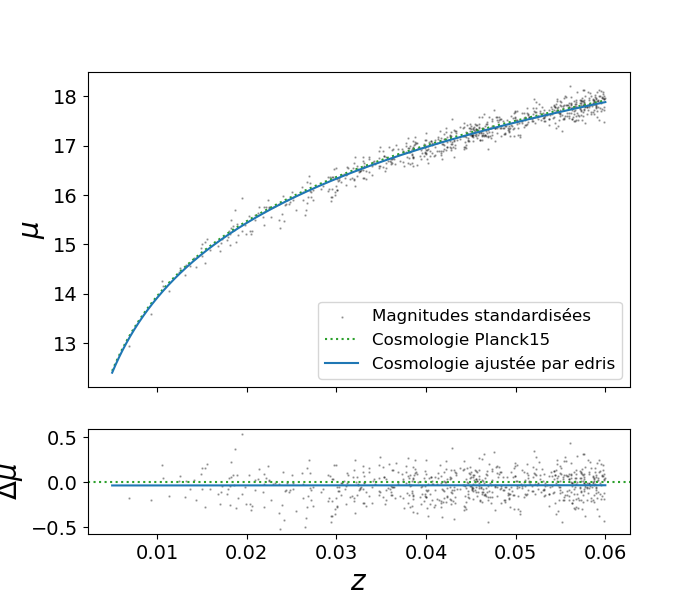
\includegraphics[width=.48\textwidth]{figures/salt_cosmo.png}
	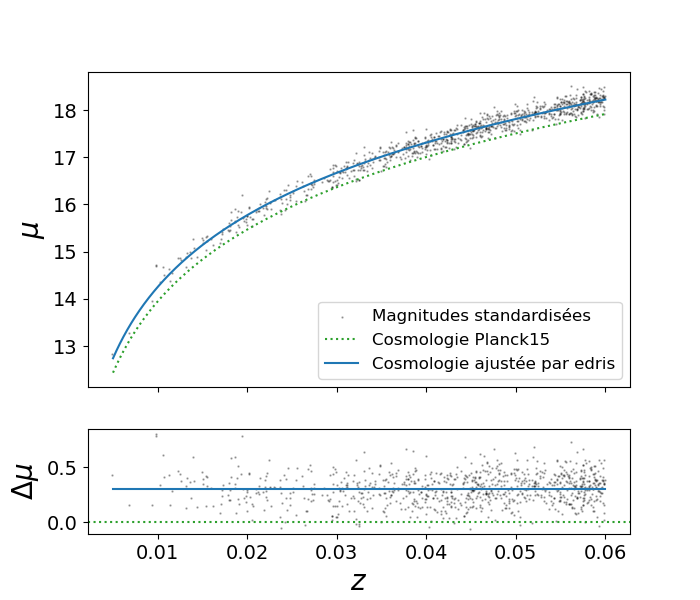
\includegraphics[width=.48\textwidth]{figures/nacl_cosmo.png}
	\caption{Modules de distance et cosmologie déterminés par \texttt{EDRIS} pour \texttt{SALT2.4} (gauche) et \texttt{NaCl} (droite)}
\end{figure}
\end{frame}

\subsection{Reconstruction des vitesses particulières}

% Préciser que c'est grâce à ZTF qu'on peut avoir des vp, car bas redshift et précision

\begin{frame}{Vitesses particulières}
Interpolation de la cosmologie $\mu(z)$ trouvée par \textit{EDRIS} pour obtenir $z(\mu)$, puis récupération des vitesses particulières par
\begin{equation}
	v_{pec} = c(z_{obs} - z(\mu))
\end{equation}
\begin{figure}
	\centering
	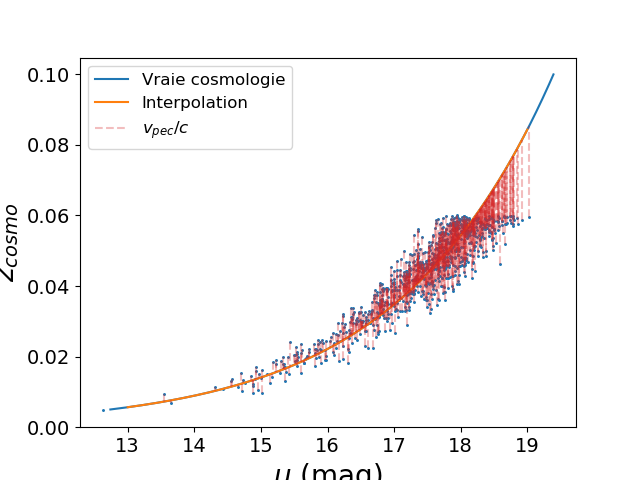
\includegraphics[width=.48\textwidth]{figures/z_mu.png}
	\caption{Inversion de $\mu(z)$ en $z(\mu)$}
\end{figure}
\end{frame}

\section{Résultats}

\subsection{Vitesses particulières obtenues}

\begin{frame}{NaCl vs Salt2.4}
\begin{figure}
	\centering
	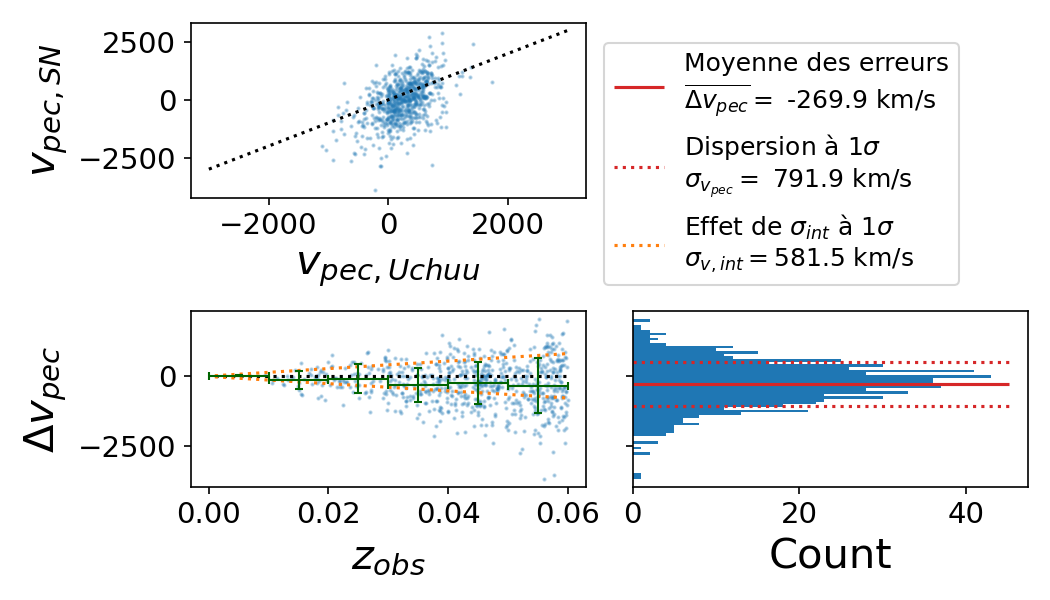
\includegraphics[width=.48\textwidth, trim = {0 0 0 0}, clip]{figures/vp_salt.png}
	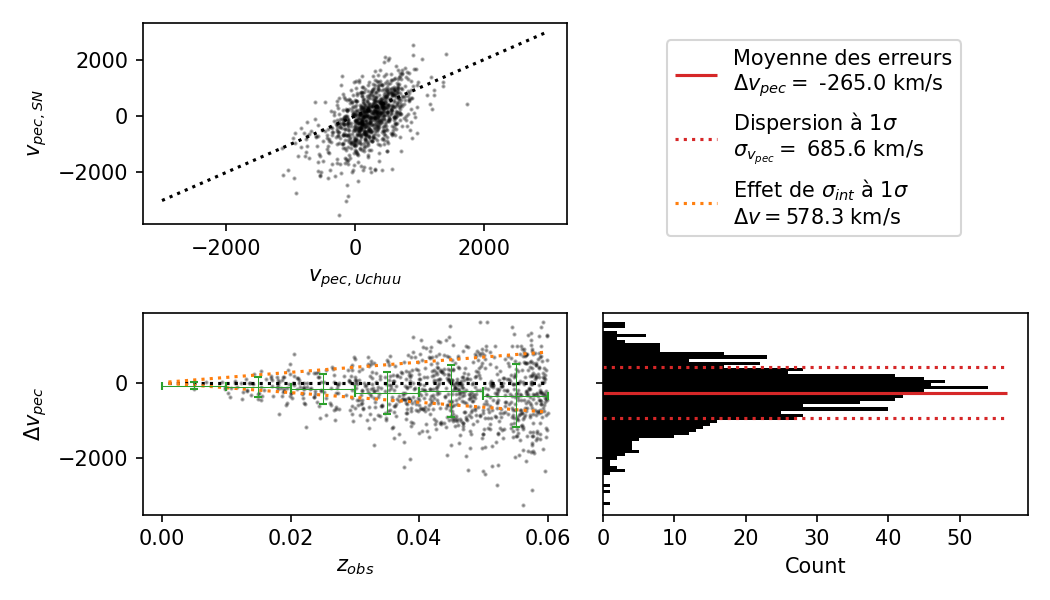
\includegraphics[width=.48\textwidth, trim = {0 0 0 0}, clip]{figures/vp_nacl.png}
	\caption{Vitesses particulières reconstruites à partir de \texttt{SALT2.4} (gauche) et \texttt{NaCl} (droite)}
\end{figure}
\end{frame}

\subsection[Contribution dans \textsc{Lemaître}]{Exemple de contribution dans la chaîne~: Réglages des hyperparamètres dans NaCl}

\begin{frame}{Réglages de hyperparamètres dans NaCl}
\only<1>{
\begin{figure}
	\centering
	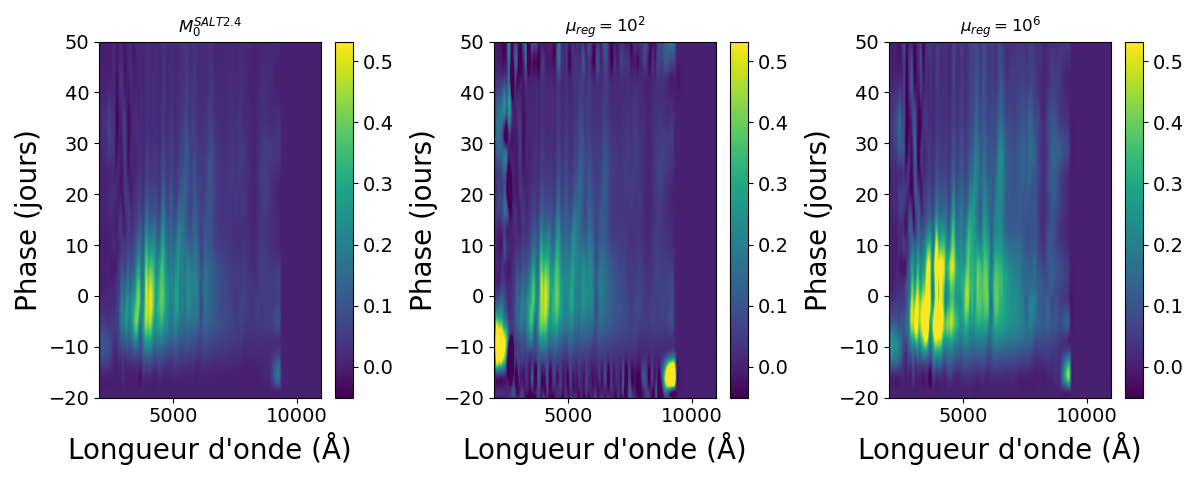
\includegraphics[width=\textwidth]{figures/mu_reg_M0.png}
	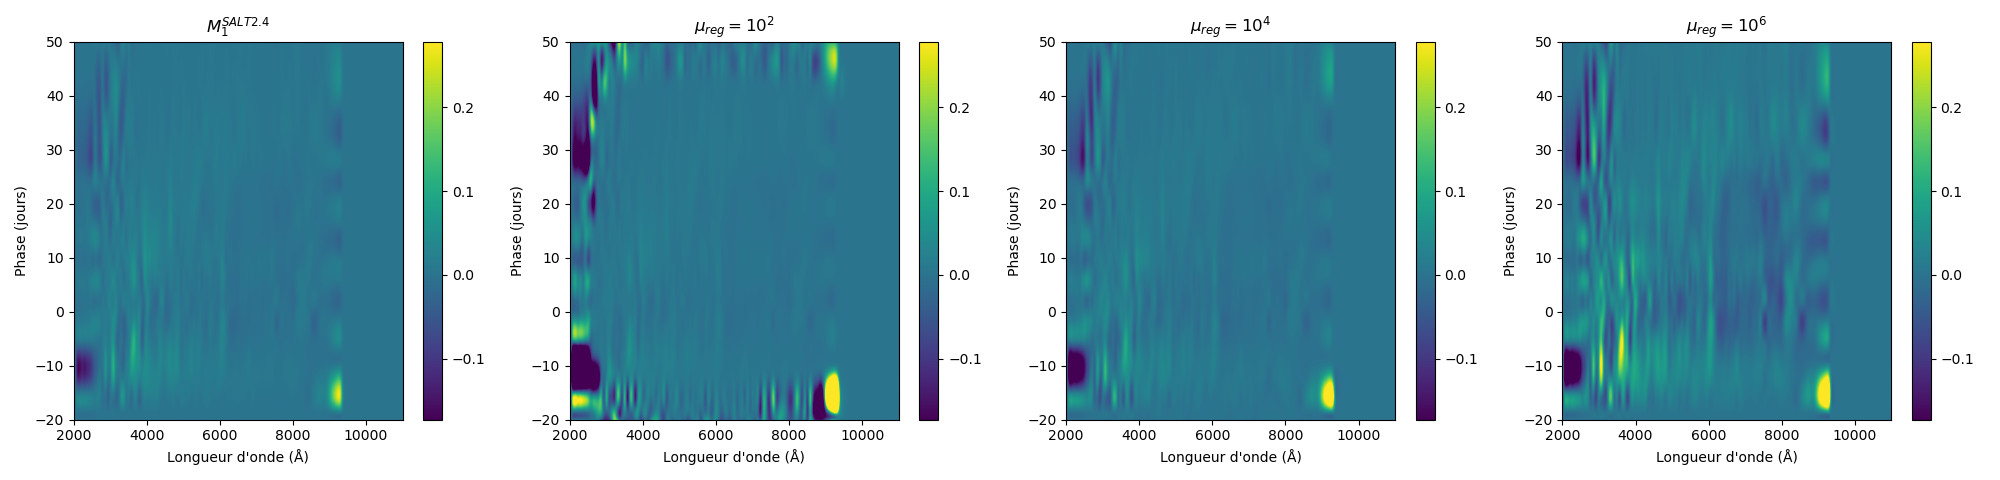
\includegraphics[width=\textwidth]{figures/mu_reg_M1.png}
	\caption{Effet de $\mu_{reg}$ sur la reconstruction des modèles}
\end{figure}}
\only<2>{
\begin{figure}
	\centering
	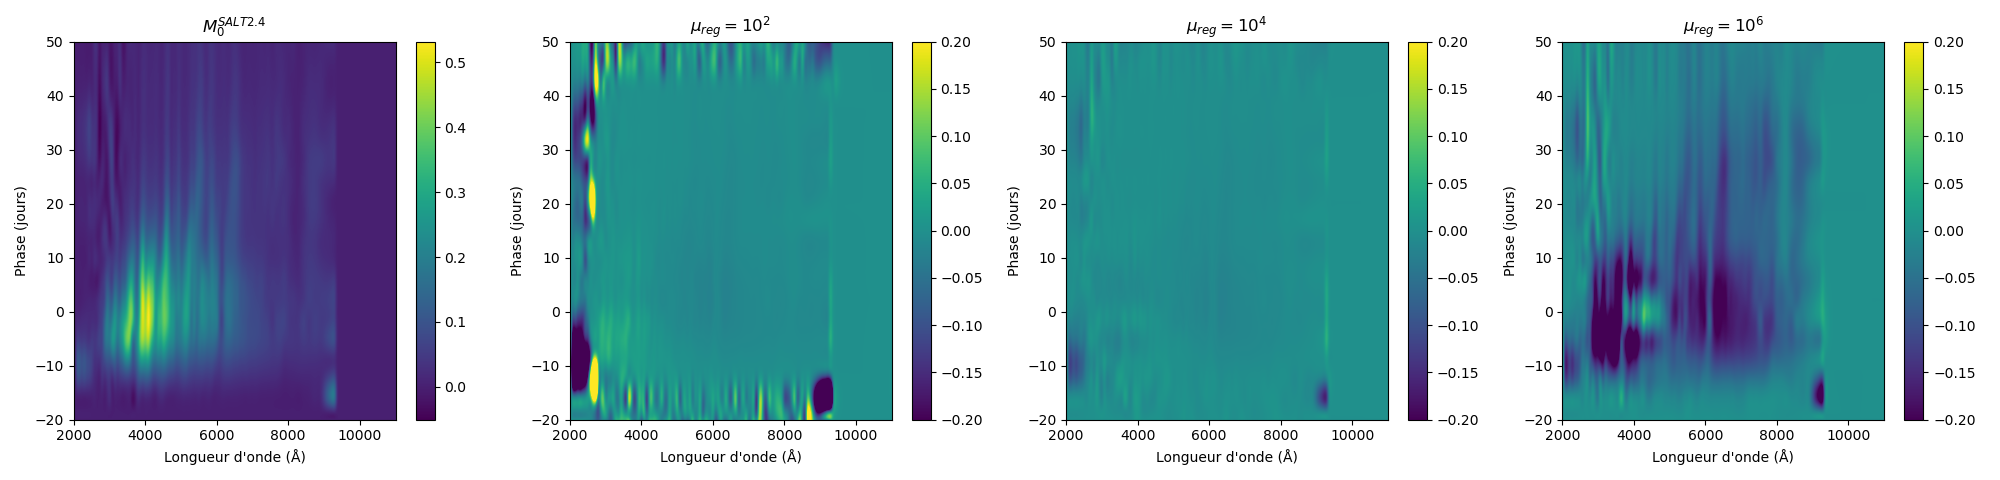
\includegraphics[width=\textwidth]{figures/mu_reg_M0_diff.png}
	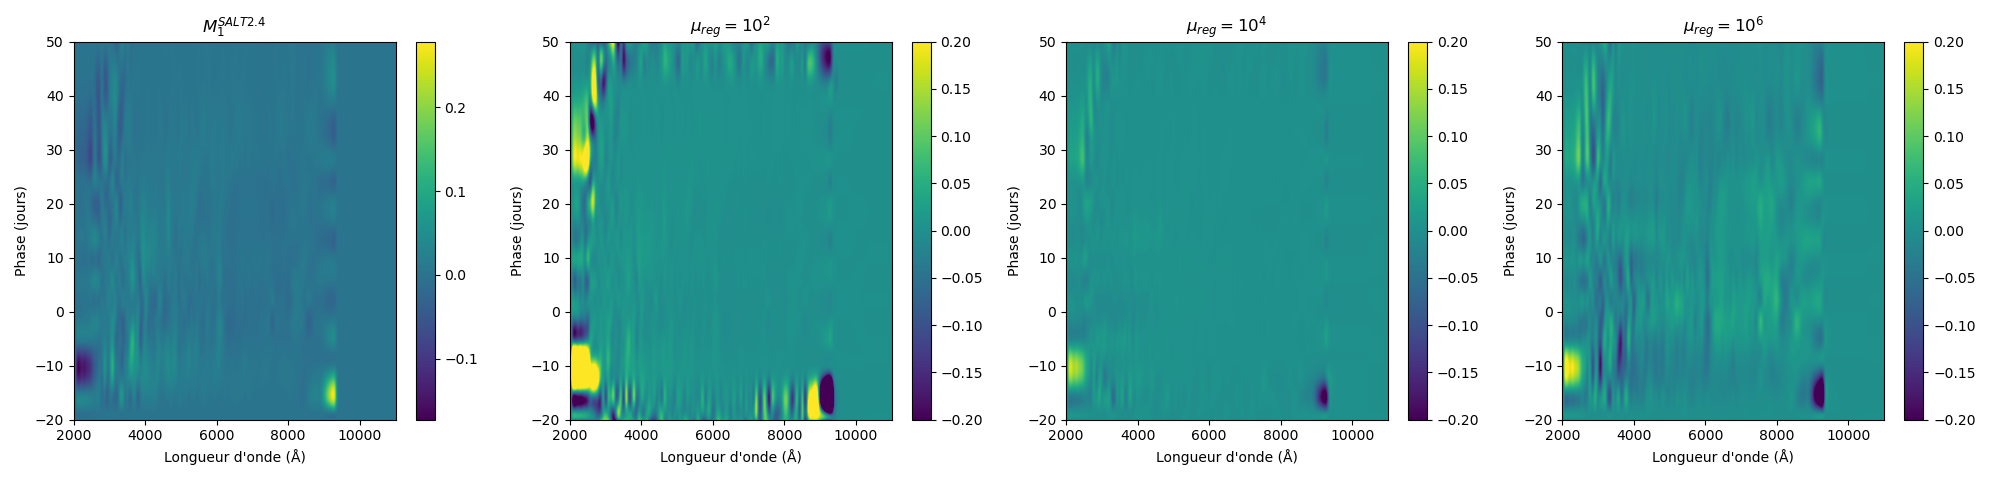
\includegraphics[width=\textwidth]{figures/mu_reg_M1_diff.png}
	\caption{Effet de $\mu_{reg}$ sur la reconstruction des modèles}
\end{figure}}
\end{frame}

% Potentiellement effet extinction galactique si implémentée d'ici-là

\section{Conclusion}

\subsection{Validation des objectifs}

\begin{frame}{Conclusion}
\begin{enumerate}
\item Possibilité de générer des SNe Ia possédant des vitesses particulières, actuellement en cours d'intégration à \texttt{skysurvey}.
\item Le pipeline \lemaitre va produire ses premiers prochainement (Data Challenge 1).
\item Les vitesses particulières sont reconstruites
\end{enumerate}
\end{frame}

\subsection{Persepctives futures}

\begin{frame}{Perspectives futures}
\begin{itemize}
\item Analyse $f\sigma_8$ utilisant un méthode de comparaison densité-vitesses
\item La génération peut utiliser n'importe quelle catalogue de galaxies, réel comme simulé
\item Permet l'étude des effets de potentielles erreurs systématiques sur les vitesses particulières
\end{itemize}
\end{frame}





\end{document}